\chapter{Overview of the State-of-the-Art Techniques} \label{chap:sota}

\minitoc

This chapter provides an objective review of the pertinent literature on \ac{DL} and audio processing. Its goal is to offer readers a comprehensive understanding of the current state of knowledge in the field and its evolution. Recent advancements in tools for sound comprehension and generation are enhancing existing models, enabling the modeling of new sounds more efficiently and rapidly~\cite{tahiroglu_-terity_2020}. Specifically, this chapter plays the following essential roles:

\begin{enumerate}
    \item To establish the context for the research problem: By reviewing the existing literature, the chapter sets the stage for the research problem and provides a basis for understanding its significance and importance.
    \item To identify gaps in the literature: The chapter helps to identify areas where further research is needed, as well as potential opportunities for contribution.
    \item To provide a foundation for the research design: The chapter helps to inform the design of the research study by highlighting previous research and its limitations.
    \item To demonstrate the originality of the research: By reviewing the existing literature, the chapter helps demonstrate the originality of the research problem and the thesis's contribution to the field.
    \item To position the thesis within the larger context of the field: The chapter helps to position the thesis within the larger context of the field, demonstrating its relevance and significance.
\end{enumerate}

The chapter is divided into two main sections: Background and Related Work. The Background section, present in \ref{sec:background}, discusses previous work that is important for understanding the context of the research problem, even though it does not address the same problem as the thesis. On the other hand, the Related Work section, present in \ref{sec:related-work}, focuses on issues that are similar or closely related to the research problem addressed in the thesis. This chapter serves as a foundation for the research problem and contributes to the overall contribution of the thesis.

\section{Background} \label{sec:background}

This dissertation is situated in a vast body of research on \ac{DL}. This section positions the current dissertation within this context. This work is not intended to explain other technologies that solve similar problems, but rather to explain other technologies that are useful in addressing the problem at hand.

The dissertation aims at readers with basic \ac{ML} knowledge, but not necessarily basics on \ac{DL}. No basis on sound besides 8th-grade physics is needed, also.

The dissertation will start by explaining how sound can be processed digitally in subsection \ref{sec:sound}, keeping this objective in mind. Then, in subsection \ref{sec:deep-learning}, it will provide a comprehensive review of general deep learning architectures and techniques, emphasizing their importance in sound synthesis. In subsection \ref{sec:parallel-tasks}, the subsequent part will concentrate on crucial techniques used in developing the suggested models. Section \ref{sec:dl-frameworks} will discuss the deep learning frameworks used in this research. Subsection \ref{sec:data-generators} will explore state-of-the-art models for data generation that are unrelated to audio but can serve as references, such as image generators, to provide further context.

\subsection{Sound} \label{sec:sound}

A digital audio signal --- often called a waveform --- captures alterations in sound pressure overtime. This waveform represents how sound waves develop and spread throughout space. Distinct sounds that constitute our auditory experience can be perceived and interpreted through analyzing the changes in frequency and amplitude within the waveform. Waveforms encode the richness of sound, enabling us to capture and manipulate it for diverse purposes such as analysis, synthesis, and artistic expression.

Sound is a continuous phenomenon but can be discretized by taking samples at a specific time rate. The number of samples taken in one second is known as the "sampling rate." The standard value for this is 44,100 Hz. The sampling rate has a direct impact on the accuracy of the signal~\cite{elsea_basics_1996}.

With the discrete version of time, it becomes possible to represent sound through an array digitally. Knowledge of the array and the sampling rate enables a computer to reconstruct the sound. These arrays can become quite large. For instance, stereo sound with a sampling rate of 44,100 \ac{Hz} needs to accommodate 1,411,200 bits per second \cite{elsea_basics_1996}.

\subsubsection{Short-Time Fourier Transform} \label{sec:stft}

Even though digital sound media can be encoded as one-dimensional data~\cite{oord_wavenet_2016}, it can be converted. By using a \acf{DFT}, the array can be represented in the frequency domain~\cite{benois-pineau_deep_2021}. Since the contents of a sound sample typically vary over time, \acp{DFT} can be computed over successive time frames of the signal. This operation forms the basis of the \acf{STFT}. The equation for \ac{STFT} is as follows:

\begin{equation} \label{eq:stft}
    STFT\{x(n)\}(m, \omega) = \sum_{n=-\infty}^{\infty} x(n) w(n - mR) e^{-j\omega n}
\end{equation}

In this equation, $STFT\{x(n)\}(m, \omega)$ represents the time-frequency representation of the input signal $x(n)$ as a function of time index $m$ and frequency $\omega$. The function is a complex-valued function containing both magnitude and phase information of the signal's frequency components at different time intervals.

The summation symbol $\sum_{n=-\infty}^{\infty}$ denotes that the product of the signal, window function, and complex exponential is summed over all time indices $n$. The discrete-time input signal is represented by $x(n)$, sampled at integer time indices $n$.

The window function, represented as $w(n - mR)$, is utilized to isolate a specific time interval of the input signal. The window function is centered at the time index $mR$, where $R$ is the hop or step size between consecutive sample windows.

Finally, the complex exponential term $e^{-j\omega n}$ is utilized to analyze the signal's frequency content within the windowed interval. The variable $j$ is the imaginary unit, and $\omega$ represents the angular frequency.

In essence, the \ac{STFT} equation computes the Fourier Transform of the input signal $x(n)$ within a windowed time interval, providing a time-frequency representation of the signal. The window function isolates a specific time interval of the signal, and the complex exponential term analyzes its frequency content. This process is repeated for different time indices $m$, resulting in a time-frequency representation that allows the study of the signal's frequency components at various time intervals.

With the \ac{STFT}, one can generate spectrograms by plotting the time in the $x$ axis and the frequency in the $y$ axis. In short, a spectrogram is a graphical representation of the frequency content of a signal over time, typically displayed as a 2D image (see Figure \ref{fig:sound} for an example).

\begin{figure}[ht]
    \centering
    \ctikzfig{figures/2-sota/sound}
    \caption[Raw Wave vs. Spectrogram]{\textbf{Raw Wave vs. Spectrogram} --- A comparative analysis of a sound sample from the Audio MNIST dataset (showcased in section \ref{sec:dataset-amnist}), specifically entry number 9 of speaker Nicolas uttering the digit ``five''. The top plot illustrates the raw waveform with time (sample rate $\times$ time) on the X-axis and energy (amplitude) on the Y-axis, providing a temporal representation of the audio signal. The bottom plot presents a spectrogram generated using the \ac{STFT} method, displaying time on the X-axis and frequency on the Y-axis, offering a time-frequency representation that reveals the spectral content and evolution of the signal over time.
    }
    \label{fig:sound}
\end{figure}

\subsubsection{Meaning of Spectrograms for Machine Learning}

Representing sound as an image opens a multitude of opportunities. However, even though spectrograms can technically be processed using \acp{CNN} (see section \ref{sec:CNN}), there is a considerable difference between a spectrogram and a standard image. In a typical image, the axes represent the same concept, the spatial position. The elements of an actual image have the same meaning independent of where they are found. A sub-object of an image does not depend on the axes. At the same time, neighbor pixels are usually highly correlated.

On the other hand, the axes of the spectrograms have different meanings \cite{benois-pineau_deep_2021}. Moving a set of pixels horizontally and vertically means different things. Therefore, structures such as \ac{CNN} are not as helpful. One can still use them but should be careful about the shape of the filters and the axis along which the convolution is performed \cite{benois-pineau_deep_2021}.

\subsubsection{Soundscapes} \label{sec:soundscapes}

The digitalization of sound has allowed for multiple applications and use cases. Applications can generate speech, and movies and videos can embed audio, such as soundscapes. Soundscapes are the sonic environments or sound environments that surround environments. They are the complex and dynamic mix of sounds heard in everyday life, including sounds from nature, human-made, and cultural sounds~\cite{international_organization_for_standardization_iso_2014, schafer_tuning_1977}. In other words, a soundscape encompasses the auditory milieu characterized by a collection of naturally occurring and human-generated sounds as perceived, encountered, and comprehended within a contextual framework by individuals. It is paramount in audio content creation, augmenting the user experience across media applications by infusing emotional engagement, a greater sense of immersion, and attention~\cite{chandrasekera_virtual_2015}.

Nevertheless, for audio media generation with \ac{ML}, one usually finds models in the literature that solve music or speech generation, not soundscapes. This is no coincidence. These sounds are more straightforward and, thus, easier to generate. Speech, for instance, usually contains a single sound source (the speaker). Also, speech and music are highly structured over time and timbrically. This happens because speech is bound to grammar, and music is bound to an underlying structure. Both of them are timbrically bound to their authors. On the contrary, soundscapes have no specific structure. Hence the increased difficulty \cite{benois-pineau_deep_2021}.

\subsection{Deep Learning}\label{sec:deep-learning}

As previously mentioned, the growth of \acf{DL} began in the early 2000s as a response to the challenge of handling vast quantities of data. Fundamentally, \ac{DL} stems from the application of \ac{ML} to process large amounts of data. To be precise, \ac{DL} is a subfield of \ac{ML} that employs multiple levels of information processing and abstraction to learn and represent features, as demonstrated by Deng et al. \cite{deng_deep_2014}. Subsequently, the extracted features can be utilized for classification, regression, and other modeling techniques. In the past, such features were manually selected by humans.

This study uses \ac{DL} for sound generation because it offers several advantages over traditional sound generation techniques. By being data-driven, these models can generate new sounds based on sounds it has heard before. On traditional methods, these sounds would have to come from the inspiration of their human creator. Besides, end-to-end generation, from text to sound generation, is only possible through \ac{DL}. The model has to extract features from the text, learn features from thousands or millions of sounds, and correlate both. This highly complex task can only be achieved with \ac{DL} techniques.

This section presents traditional \ac{DL} architectures and their evolution to generative \ac{DL} architectures.

%%%%%%%%%%%%%%%%%%%%%%%%%%%%%%%%%%%%%%%%%%%

\subsubsection{Deep Learning Architectures}

Generative \ac{DL} architectures establish blueprints for developing \ac{DL} networks that synthesize diverse and novel data samples according to a learned distribution. These architectures entail creating latent data constructs and learning to emulate the fundamental statistical patterns found in observed data.

Generative deep neural models have been applied to tasks comprising image synthesis, text generation, and audio synthesis. Their popularity has recently surged owing to their remarkable ability to generate high-quality data and effectively model complex distributions. In the following sections, we outline the most ordinarily used generative \ac{DL} architectures, presented chronologically, as summarized in Table~\ref{tab:archs}.

\begin{table*}[ht]
\centering
\caption{Comparison of Generative Deep Learning Architectures}
\label{tab:archs}
\begin{tabularx}{\textwidth}{|p{20mm}|c|p{25mm}|X|c|}
\hline
\textbf{Model} & \textbf{Year} & \textbf{Type} & \textbf{Key Characteristics} & \textbf{Inference} \\ \hline
DARN & 2013 & Autoregressive & Uses a single model to predict the probability distribution of each output token conditioned on the previous tokens & Sequential \\ \hline
VAE & 2013 & Variational Autoencoder & Learns a latent representation of the input data and generates new samples by sampling from the learned latent space & Parallel \\ \hline
GAN & 2014 & Generative Adversarial Network & Consists of a generator and a discriminator that compete in a two-player minimax game to generate realistic samples & Parallel \\ \hline
Normalizing Flows & 2015 & Flow-based models & Transforms a simple probability distribution into a complex one by applying a sequence of invertible transformations & Parallel \\ \hline
Diffusion & 2015 & Flow-based models & Uses a diffusion process to model the probability distribution of the data & Parallel \\ \hline
Transformers & 2017 & Attention-based models & Uses self-attention to capture global dependencies and generate sequences & Sequential \\ \hline

VQ-VAE &
    2018 &
    Variational Autoencoder &
    Discretizes the continuous latent space by mapping each latent vector to the closest codebook vector &
    Parallel \\ \hline

MS-VQ-VAE &
    2019 &
    Variational Autoencoder &
    Is an extension of the VQ-VAE that incorporates multiple discrete latent spaces of different scales, enabling hierarchical and diverse representations with improved abstraction levels and latent space expressiveness &
    Parallel \\ \hline

\end{tabularx}
\end{table*}

This section will discuss novel architectural designs for \ac{DL}. It is important to note that there is a discrepancy between the date of their conceptualization and their widespread adoption. This trend is common in machine learning because software theories have a faster rate of development compared to hardware theories.

This section does not describe all \ac{DL} architectures that had some relevance. It, however, describes the ones used either by the models developed or by systems studied for the state-of-the-art.

\input{src/chapters/2-state-of-the-art/background/deep-learning-models/deep-learning/feedforward}
\input{src/chapters/2-state-of-the-art/background/deep-learning-models/deep-learning/cnn}
\input{src/chapters/2-state-of-the-art/background/deep-learning-models/deep-learning/conv-layers}
\input{src/chapters/2-state-of-the-art/background/deep-learning-models/deep-learning/rnn}
\input{src/chapters/2-state-of-the-art/background/deep-learning-models/deep-learning/rnn-variants}
\input{src/chapters/2-state-of-the-art/background/deep-learning-models/deep-learning/ae}
\input{src/chapters/2-state-of-the-art/background/deep-learning-models/deep-learning/u-net}
\subsubsection{Foundations of Deep Learning} \label{sec:dl-foundations}

This section explores the fundamental principles of \ac{DL}, with a specific focus on activation functions and backpropagation. Activation functions play a vital role in neural networks by introducing non-linearity and enabling the representation of complex relationships. This section covers the most commonly used activation functions. In addition, this section discusses the backpropagation algorithm, which plays a crucial role in training feedforward neural networks by calculating gradients with respect to network weights for iterative adjustments and optimal model performance. Furthermore, this section explores optimization techniques within deep learning.

\input{src/chapters/2-state-of-the-art/background/deep-learning-models/dl-basics/activation}
\input{src/chapters/2-state-of-the-art/background/deep-learning-models/dl-basics/backpropagation}
\input{src/chapters/2-state-of-the-art/background/deep-learning-models/dl-basics/sgd}
\input{src/chapters/2-state-of-the-art/background/deep-learning-models/dl-basics/adam}
\subsubsection{Generative Deep Learning Architectures}

Generative \ac{DL} architectures are a subset of \ac{DL} networks designed to generate new and diverse data samples from a learned distribution.

By finding latent data structures and learning to reproduce the hidden statistics behind observed data, they do so. To achieve this, the model tries to estimate an underlying probability distribution $p_{data}$ when given a set of samples from this distribution. Thus, training a generative model involves selecting the best parameters that reduce some concept of distance/loss/error between the model and the actual distribution. As Huzaifah \cite{huzaifah_deep_2021} states: ``given training data points $X$ as samples from an empirical distribution $p_{data}(X)$, we want to learn a model $p_\theta(X)$, belonging to a model family $M$ that closely matches $p_{data}(X)$, by repeatedly changing model parameters $\theta$''. This is expressed as the problem in equation \ref{eq:generative-models-base}.

\begin{equation} \label{eq:generative-models-base}
    \min_{\theta \in M} d (p_{data}, p_\theta)
\end{equation}

Standard functions for $d$ are displayed in section \ref{sec:loss-functions}.

These models have been applied to various tasks, such as image synthesis, text generation, and audio synthesis. Generative \ac{DL} models have gained popularity recently due to their ability to produce high-quality data and model complex distributions.

This section will present the most used architectures.

\input{src/chapters/2-state-of-the-art/background/deep-learning-models/generative/darn}
\input{src/chapters/2-state-of-the-art/background/deep-learning-models/generative/vae}
\input{src/chapters/2-state-of-the-art/background/deep-learning-models/generative/gan}
\input{src/chapters/2-state-of-the-art/background/deep-learning-models/generative/flow}
\input{src/chapters/2-state-of-the-art/background/deep-learning-models/generative/diffusion}
\input{src/chapters/2-state-of-the-art/background/deep-learning-models/generative/transformers}
\input{src/chapters/2-state-of-the-art/background/deep-learning-models/generative/vq-vae}
\input{src/chapters/2-state-of-the-art/background/deep-learning-models/generative/ms-vq-vae}
\subsection{Foundations for Enhancing Generative Models for Audio} \label{sec:parallel-tasks}

To develop generative models for audio, it is necessary to address several factors that impact their performance and quality. This thesis concentrates on three main areas: data augmentation, evaluation metrics, and data embedding.

\textit{Data augmentation} is the process of applying transformations to the original data to increase its size and diversity. This can help overcome the limitations of small or imbalanced datasets and improve the generalization ability of generative models. Different types of data augmentation techniques for sound generation and their effects on the model outcomes are discussed in Sextion \ref{sec:data-augmentation}.

\textit{Evaluation metrics} are the methods used to measure the quality and diversity of the generated sounds. They provide a way to compare different generative models and assess their strengths and weaknesses. However, evaluating sound generation is not trivial, as it involves objective and subjective criteria. We review various evaluation metrics for sound generation and their advantages and disadvantages in Section \ref{sec:evaluation}

\textit{Data embedding} is the technique of converting data into numerical representations that capture its essential features and characteristics. This can facilitate the learning process of generative models and enhance their expressiveness and efficiency. We explore different data embedding methods in section \ref{sec:text-embedding}.

\subsubsection{Data Augmentation} \label{sec:data-augmentation}

Data augmentation is crucial to \ac{ML} tasks. It helps to increase the training dataset's size and improve the model's robustness. For the task at hand, there are two main types of data augmentation: acoustic and linguistic. Data augmentation can reduce overfitting and improve generalization by introducing more variations into the training set~\cite{pluscec_data_2023}.

\input{src/chapters/2-state-of-the-art/background/more/data-augmentation/acoustic-augmentation}
\input{src/chapters/2-state-of-the-art/background/more/data-augmentation/linguistic-augmentation}
\subsubsection{Evaluation Metrics} \label{sec:evaluation}

The evaluation process can provide insights into the system's performance and reveal areas that need improvement. Moreover, a proper evaluation metric helps to compare the results of different models and choose the best one. The aim of this section is to provide a comprehensive overview of the available evaluation metrics for audio generation and to provide a foundation for the evaluation of the system developed in this thesis.

In this thesis, a comprehensive evaluation framework is developed that considers two different types of evaluations. The first type of evaluation focuses on metrics that can be used for training models offline, such as loss metrics, which play a crucial role in assessing the performance of a model. The second type of evaluation focuses on evaluating the broader impacts of a model, such as its environmental impact and inference time for a generation. These evaluations are essential in ensuring that the model not only performs well on its primary task but also has minimal negative impacts on other aspects of the system.

\paragraph{Loss Functions} \label{sec:loss-functions}

Evaluating generative audio systems is challenging due to the need for a standard set of metrics to capture the quality and diversity of the generated audio samples. Different studies often use different evaluation methodologies and metrics when reporting results, making a direct comparison to other systems intricate if not impossible~\cite{vinay_evaluating_2022}. Furthermore, the perceptual relevance and meaning of the reported metrics, in most cases unknown, prohibit any conclusive insights concerning practical usability and audio quality.

A review and comparison of the available evaluation metrics for audio generation is essential to provide a foundation for evaluating the system developed in this thesis. This section discusses some of the commonly used metrics for evaluating generative audio systems, such as \ac{MAE}, \ac{MSE}, \ac{KL} divergence, and \ac{ELBO}. It also discusses their advantages and limitations and how they can be applied to sound generation tasks.

\subparagraph{Mean Absolute Error} \label{sec:mae}

The \Acf{MAE} is a quantitative measure of the average magnitude of the errors between the predicted and actual values~\cite{willmott_advantages_2005}. It is computed as:

\begin{equation}
	\text{MAE} = \frac{1}{n} \sum_{i=1}^n |y_i - \hat{y}_i| 
\end{equation}

where $y_i$ denotes the true value, $\hat{y}_i$ denotes the predicted value, and $n$ denotes the number of samples. The \ac{MAE} is also called L1-norm loss or \acf{MAD}.  

The \Ac{MAE} is a relevant metric for evaluating generative models as it treats all errors equally and is arguably less sensitive to outliers compared to \ac{MSE} (see Section \ref{sec:mse}). Specifically, it indicates the average absolute difference between the predicted and actual values in the same unit as the output.

However, the \ac{MAE} has some notable limitations that should be considered. For instance, it does not directly capture the perceptual quality of the generated audio samples. The perceptual quality of audio can depend on factors such as timbre, pitch, or harmony, which are not explicitly determined by the \ac{MAE}. Therefore, to fully assess the quality of generative models, the \ac{MAE} should be complemented with other metrics and human evaluation. Additionally, the \ac{MAE} is a scale-dependent measure and cannot be used to compare predictions that use different scales.

To illustrate the difference between \ac{MAE} computed on raw audio versus spectrograms, consider the following example: For a 1D raw audio sample, the \ac{MAE} would measure the average absolute difference between the amplitude values of the audio signals. In contrast, if the audio data were represented as spectrograms, the \ac{MAE} would measure the average absolute difference between the magnitude values of the frequency bins. In this case, the spectrograms can be treated as images with a single channel, and the \ac{MAE} can be seen as a pixel-wise error metric.  

It is important to consider the limitations of the \ac{MAE} when evaluating generative models. For example, consider a scenario with two audio samples of a dog barking: one with a bark at one second and another with a bark at two seconds. Despite being similar sounds with different temporal positions, calculating their \ac{MAE} would lead to higher-than-expected error as it does not account for temporal alignment. Therefore, it is important to use other metrics and human evaluation methods along with \ac{MAE} to assess timing accuracy and perceptual quality of generated audio samples comprehensively.

\subparagraph{Mean Squared Error} \label{sec:mse}

\Acf{MSE} is a standard metric to evaluate the performance of a predictor or an estimator. It quantifies the average of the squared errors, the average squared difference between the estimated and actual values. \Ac{MSE} is always a non-negative value approaching zero as the error decreases. The smaller the \ac{MSE}, the better the predictor or estimator~\cite{hodson_mean_2021}.

\Ac{MSE} can be calculated as follows:

$$
MSE = \frac{1}{n} \sum_{i=1}^n (y_i - \hat{y}_i)^2
$$

Where $n$ is the number of data points, $y_i$ is the true value of the variable being predicted or estimated, and $\hat{y}_i$ is the predicted or estimated value.

\Ac{MSE} incorporates both the variance and the bias of the predictor or estimator. The variance measures how widely spread the estimates are from one data sample to another. The bias measures the distance of the average estimated value from the true value. For an unbiased estimator, the \ac{MSE} equals the variance.

\Ac{MSE} can compare different predictors or estimators and select the one that minimizes the \ac{MSE}. For instance, in linear regression, \ac{MSE} can be used to find the best-fitting line that minimizes the sum of squared errors. \Ac{MSE} can also evaluate the quality of a generative model that produces audio samples from textual input. In this case, \ac{MSE} can measure how similar the generated audio samples are to the target audio samples regarding their amplitude values.

Unlike \ac{MAE} (see Section \ref{sec:mae}), which assigns equal weight to all errors, \ac{MSE} penalizes larger errors more than smaller ones. This means that \ac{MSE} is more sensitive to outliers and may not reflect the overall discrepancy between the generated and target audio samples well. Moreover, \ac{MSE} does not account for perceptual aspects of audio quality, such as timbre, pitch, or loudness. Therefore, \ac{MSE} should be used with other metrics and evaluation methods, such as \ac{KL} divergence (see Section \ref{sec:kld}), subjective listening tests, or qualitative analysis.

\Ac{MSE} can be applied to sound generation tasks in different ways, depending on the representation of the audio data. Similar to \ac{MAE}, it can be applied to 1D raw audio and spectrograms.

It should be noted that \ac{MSE} is subject to the same temporal issue as \ac{MAE}. \Ac{MSE} may not be effective in identifying differences in timing accuracy. Therefore, it is crucial to employ other metrics and evaluation methods that specifically focus on timing aspects and perceptual quality when assessing audio produced by text-trained models.

\subparagraph{Cross-Entropy} \label{sec:cross-entropy}

Cross Entropy Loss is commonly used to evaluate \ac{DL} models, especially in classification or sequence generation tasks. It measures the dissimilarity between predicted and target distributions by calculating the average negative log-likelihood of predicting each class or element correctly.

Cross Entropy Loss can be applied in audio generation tasks to produce discrete elements, such as musical notes or phonemes. For instance, if one aims to create music based on textual input with particular note sequences, Cross Entropy Loss can assess the prediction accuracy of each note at every time step.

Mathematically, given data samples $x_i$ and their respective true labels $y_i$, where $i$ ranges from 1 to $n$, Cross Entropy Loss can be calculated in the following way:

\begin{equation}
    CE = -\frac{1}{n}\sum_{i=1}^{n} \sum_{j=1}^{C} y_{ij}\log(p_{ij})
\end{equation}

This is where:
The symbol $C$ represents the number of classes or elements.
The notation $y_{ij}$ indicates whether sample $x_i$ belongs to class $j$ (or has element $j$).
Additionally, $p_{ij}$ represents the predicted probability that sample $x_i$ belongs to class $j$ (or has element $j$).

The objective is to minimize the Cross Entropy Loss during training, so that the generative model can learn to predict precise and coherent distributions over classes or elements.

Nonetheless, it is important to consider some limitations when using Cross Entropy Loss to evaluate audio generation systems. First, the model assumes independence between individual predictions within one sample. However, this assumption may not hold for sequential audio data where the context and dependencies between elements are critical. Second, the Cross Entropy Loss does not directly capture perceptual aspects of audio quality, such as timbre or tonality. Therefore, it is advisable to combine Cross Entropy Loss with other evaluation metrics, such as \ac{MAE}, \ac{MSE}, or subjective listening tests to achieve a comprehensive understanding of the generative model's performance.

To summarize, the Cross Entropy Loss is commonly employed as a loss function for evaluating generative models that involve discrete element generation. Although it is applicable for audio generation tasks with categorical outputs such as music note prediction, it should be combined with other evaluation methods to gain a more comprehensive assessment of accuracy and perceptual quality.

\subparagraph{KL Divergence} \label{sec:kld}

\acf{KL} divergence, also known as relative entropy, is a non-symmetric measure of the difference between two probability distributions. It is a mathematical quantity that quantifies the distance between two probability distributions.

In simple terms, \ac{KL} divergence measures the difference between the probability distribution predicted by a model and the true underlying distribution of the data. \Ac{KL} divergence is commonly used to evaluate generative models.

\ac{KL} divergence is calculated as the expectation of the logarithmic difference between the predicted probability distribution and the actual distribution. It is a scalar value, and the smaller the \ac{KL} divergence, the closer the predicted distribution is to the real distribution.

The \ac{DL} system can be trained to produce sounds near the target sounds in terms of their probability distribution by using \ac{KL} divergence as a loss function. The concept is that the sound does not have to be alike the input, but only its distribution. Maximizing the log-likelihood between the generated output and the given input can be seen as minimizing the \ac{KL} divergence \cite{huzaifah_deep_2021}.

\subparagraph{Evidence Lower Bound (ELBO)} \label{sec:elbo}

\Acf{ELBO} is a lower bound on the log-likelihood of some observed data commonly used in variational Bayesian methods \cite{blei_variational_2017}.

The \ac{ELBO} is defined as follows:

\begin{equation}
ELBO = E_{Z \sim q}\left[\log \frac{p(X,Z; \theta)}{q(Z)} \right]
\end{equation}

where $X$ and $Z$ are random variables with joint distribution $p(X,Z; \theta)$, $\theta$ are the parameters of the model, and $q(Z)$ is an approximate posterior distribution for the latent variable $Z$. The \ac{ELBO} can be seen as the difference between two terms: the expected log joint probability of the data and the latent variables under the model and the entropy of the approximate posterior distribution.

The \ac{ELBO} has several desirable properties. First, it is a lower bound on the log-likelihood of the data, $\log p(X; \theta)$, also known as the evidence. Meaning that the \ac{ELBO} is a quantity that is always less than or equal to the log-likelihood of the data, which is the logarithm of the probability of the data given the model parameters. The log-likelihood of the data is also called the evidence because it indicates how well the model fits the data. The higher the log-likelihood, the more evidence we have that the model is suitable for the data. However, computing the log-likelihood of the data is often intractable. Therefore, the model can be optimized more easily using \ac{ELBO}.

Second, it is a tractable objective function that can be optimized concerning $\theta$ and $q(Z)$. This allows us to perform variational inference, approximating the posterior distribution $p(Z|X; \theta)$ by finding the $q(Z)$ that maximizes the \ac{ELBO}. This can be done using gradient-based methods, thus being used in machine learning systems.

Third, it can be decomposed into two significant components: the reconstruction term and the regularization term. The reconstruction term is the expected log-likelihood of the data given the latent variables under the model, $E_{Z \sim q}\left[\log p(X|Z; \theta)\right]$. It measures how well the model fits the data. The regularization term is the negative \ac{KL} divergence (see section \ref{sec:kld}) between the approximate posterior and the prior distributions, $-D_{KL}(q(Z)||p(Z))$. It measures how close the approximate posterior is to the prior. The \ac{KL} divergence is always non-negative, and it is zero if and only if $q(Z) = p(Z)$. Therefore, maximizing the \ac{ELBO} encourages data fidelity and posterior regularization.

The \ac{ELBO} can be applied to sound generation tasks using a deep generative model such as a \ac{VAE} (see section \ref{sec:vae}). This model can be trained by maximizing the \ac{ELBO} concerning its parameters and latent variables. The \ac{ELBO} can then be used to evaluate the quality and diversity of the generated sounds by comparing them to the target sounds. For instance, the \ac{ELBO} for a \ac{VAE} can be written as:

\begin{equation}
ELBO = E_{Z \sim q_\phi(Z|X)}\left[\log p_\theta(X|Z)\right] - D_{KL}(q_\phi(Z|X)||p(Z))
\end{equation}

The first term is the reconstruction term, which measures how well the decoder network reconstructs the input sound $X$ from the latent variable $Z$. The second term is the regularization term, which measures the proximity of the approximate posterior distribution to a prior distribution $p(Z)$.

By maximizing the \ac{ELBO}, a model learns to generate realistic sounds similar to the input sounds regarding their conditional distribution while ensuring that the latent variables have a smooth and regular structure that facilitates interpolation and manipulation.

\paragraph{Model Evaluation Functions}

The second type of evaluation in this thesis involves assessing the wider impacts and implications of the developed audio generation model. Although metrics used for training models offline provide insights into performance, it is equally important to evaluate how a model affects aspects beyond its primary task. This includes considerations such as the environmental impact and inference time during generation, among others. Understanding these broader impacts ensures that the model not only performs well in its intended purpose but also operates with minimal negative consequences or trade-offs in other areas of the system. Conducting evaluations encompassing these factors will provide a more comprehensive understanding of how well-rounded and sustainable our audio generation system is.

\subparagraph{Evaluating Energy Expended}

Evaluating the amount of energy expended by a deep learning model is crucial in developing and deploying these systems. With the increasing demand for machine learning applications and the complexity of deep learning models, energy efficiency has become a critical factor in designing and deploying deep learning systems.

With the growing concern for environmental sustainability, the energy footprint of deep learning models has become an essential topic in the field. Most of the recent advances produced by deep learning approaches rely on significant increases in size and complexity \cite{douwes_energy_2021}. Such improvements are backed by an increase in power consumption and carbon emissions. The high energy consumption of deep learning models during both the training and inference phases significantly impacts the environment, and it is imperative to address this issue.

Therefore, evaluating the amount of energy a deep learning model expends is essential in ensuring its practicality and scalability. This is a crucial step in ensuring that the deep learning models developed today are not only accurate, but also energy-efficient and sustainable for future deployment.

This evaluation can be done in two ways: physically measuring the energy expended by the machines on both learning and inference time or by approximating given average numbers per neuron, for instance.

A good model is a compromise between accuracy and complexity. If the model trains significantly longer to train or infer and does not provide way better results, in the context of this research, the model is not much better than a simpler counterpart.
\subsubsection{Data Embedding} \label{sec:text-embedding}

Data embedding is the technique of converting data into numerical representations that capture its essential features and characteristics. For sound generation, both audio and text embedding is important.

Data embedding is essential for generative models. This happens for two reasons.

First, it allows the models to work on smaller and lighter representations. This is, for instance, taking an audio sample with 5 seconds sampled at 16 kHz, representing 80 000 entries. Encoding that into meaningful features might reduce this number to a few thousand or even hundreds of entries. This allows for faster training.

Second, these representations are meaningful in ways where the raw input is not. For instance, take text embedding. The idea is that words such as ``pretty'' and ``beautiful'' have similar representations, helping the model generalize. If the model were to check the words, letter by letter, it would have a hard time realizing that some words, like these, have a relation between them.

So, text and audio embedding is essential for the task. However, audio embedding possesses several challenges, such as dealing with high-dimensional and sequential data, preserving temporal and spectral information, and ensuring robustness and interpretability. To handle this, both feature and learning-based methods can be applied.

Feature-based embedding methods extract predefined features from the raw audio data, such as spectral, temporal, or perceptual features. These features are then input to generative models or further processed to obtain lower-dimensional embeddings. One such example would be the application of the \ac{STFT} to build a spectrogram (see Section \ref{sec:sound}). Feature-based embedding methods have the benefit of being simple and interpretable, but they may also lose some information or introduce noise during the feature extraction process.

Using neural networks or other machine learning techniques, learning-based embedding methods learn embeddings directly from the raw audio data. These methods can automatically discover relevant features from the data without relying on predefined criteria. Learning-based embedding methods have the advantage of being flexible and adaptive, but they may also require more computational resources or suffer from overfitting or underfitting issues.

Text embedding has been a solved problem since the days of Word2Vec \cite{mikolov_efficient_2013}. This \ac{AE} (see Section \ref{sec:autoencoders}) model would be trained by getting the meaning of a word taking into account the word with whom the first appeared. This model makes possible the representation of a word through a vector of latent factors.

Nevertheless, the words cannot be merely embedded for the current issue. When a user adds a text input, embedding it is imperative. This represents the entire textual input. For example, computing the average of latent factors for each input would be a naive approximation.

Nevertheless, nowadays, this is mainly solved with transformers (see Section \ref{sec:transformers}), namely the encoder part. This part of the transformer takes a whole string and outputs a vector representation, precisely what the task needs.

After the vanilla transformer, the one that gained more prominence was BERT \cite{devlin_bert_2018} in 2018, which introduced the conditioning of the whole input for each word inputted, not only the words that appeared before, as the vanilla transformer did. Other later encoder transformers are based on BERT or tackle a different problem.

While there are many techniques for data embedding, recent advancements in the field have led to the development of specialized models for various modalities, such as CLIP \cite{radford_learning_2021} for images and MuLan for audio. Instead of embedding the text and the media separately and dealing with it afterward, media and text are embedded in the same space, meaning that a textual segment and a media sample representing the same textual segment should have similar latent factors.

\paragraph{MuLan} \label{sec:mulan}

MuLan \cite{huang_mulan_2022} is a state-of-the-art music audio embedding model that aims to link music audio directly to unconstrained natural language music descriptions.

MuLan employs a two-tower parallel encoder architecture, meaning two completely independent neural architectures, using a contrastive loss objective that elicits a shared embedding space between music audio and text.

Each MuLan model consists of two separate embedding networks for the audio and text input modalities. These networks share no weights, but each terminates in 2-normalized embedding spaces with the same dimensionality. The contrastive loss objective minimizes the distance between matching audio-text pairs while the distance between mismatched pairs is maximized. This approach enables MuLan to learn a joint representation of music audio and text that captures their semantic relationships.

MuLan is trained using 44 million music recordings (370K hours) and weakly-associated, free-form text annotations. The resulting audio-text representation subsumes existing ontologies while graduating to true zero-shot functionalities. MuLan demonstrates versatility in transfer learning, zero-shot music tagging, language understanding in the music domain, and cross-modal retrieval applications.
 \subsection{Deep Learning Frameworks} \label{sec:dl-frameworks}

\Ac{DL} frameworks have revolutionized the field of \ac{AI}, enabling researchers and practitioners to efficiently develop and deploy complex neural networks for the multiple \ac{DL} tasks. These frameworks provide a wide range of tools and techniques for building, training, and evaluating deep neural networks and have significantly accelerated the pace of progress in the field. This section explores some of the most popular \ac{DL} frameworks, their key features and capabilities, and how they have been used to develop state-of-the-art generative \ac{AI} models for audio synthesis from textual input.

Several \ac{DL} frameworks are available, and they differ in several ways, including their programming languages, ease of use, and performance. However, to the best of the author's knowledge, there is no recent study on the performance of today's \ac{DL} networks. The most recent is from 2017 \cite{parvat_survey_2017}.	

\subsubsection{TensorFlow} \label{sec:tensorflow}

Developed by Google, TensorFlow \cite{martin_abadi_tensorflow_2015} is one of the most widely used \ac{DL}. It supports both \ac{CPU} and \ac{GPU} computations and provides a variety of \acp{API} for building different types of neural networks. TensorFlow is written in Python, but its core functionality is implemented in C++ for optimal performance.

TensorFlow is an interface for expressing \ac{ML} algorithms and an implementation for executing them. It allows computations to be executed with little or no change on various systems, from mobile devices to large-scale distributed systems. The system is flexible and can express many different algorithms, including training and inference algorithms for deep neural network models.

TensorFlow can be used with various programming languages, including Python, JavaScript, C++, and Java. Python is the recommended language for TensorFlow, but other languages' \acp{API} may offer some performance advantages. Other languages like Julia, R, Haskell, and others have bindings.

\subsubsection{PyTorch} \label{sec:pytorch}

PyTorch is an open-source \ac{DL} framework developed by Facebook \cite{paszke_pytorch_2019}. It has gained popularity due to its ease of use and dynamic computation graph, which allows for more flexible and intuitive programming. PyTorch also supports \ac{CPU} and \ac{GPU} computations, and although it supports Python and C++, it has a Python-first approach, making it easy to integrate with other Python libraries.

PyTorch is a popular deep-learning framework that is easy to use and learn. It has a simple and intuitive \ac{API} that makes it easy to learn and use. PyTorch is also flexible and can be used for various applications.

\subsubsection{Keras} \label{sec:keras}

Keras is a Python library for building and training neural network models at a high-level. It offers a user-friendly interface, and it is commonly used for \ac{DL} purposes~\cite{chollet_keras_2015}. Keras is built on top of lower-level libraries such as TensorFlow (see Section~\ref{sec:tensorflow}). It simplifies the creation and training of neural networks by abstracting away many low-level details.
Keras enables fast neural network model creation by assembling pre-built building block layers. These building blocks consist of input layers, \ac{CNN} layers, \ac{RNN} layers, fully connected layers, activation functions, and other components.

Keras is often regarded as more user-friendly than TensorFlow, as it offers a high-level interface that hides many low-level details.

Keras provides a simplified \ac{API} for constructing and training deep learning models. Keras includes a variety of utilities for manipulating data, such as data preprocessing, data augmentation, and data visualization, facilitating data manipulation.

\subsubsection{Conclusions on Deep Learning Frameworks} \label{sec:dl-frameworks-conclusions}

Selecting a \ac{DL} framework is critical in developing a \ac{DL} project. It is vital for the development of this thesis that the best framework that can offer flexibility, ease of use, and optimal performance of the \ac{DL} models is selected.

PyTorch uses a dynamic computation graph, which is created for each iteration in an epoch. In each iteration, the code executes the forward pass, computes the derivatives of output \textit{w.r.t} to the network parameters, and updates the parameters to fit the given examples. After doing the backward pass, the graph is freed to save memory. A dynamic graph can be changed on the fly, allowing for more freedom, easier debugging, and easier experimentation with architectures and hyperparameters during the model development process. Tensorflow, on the other hand, uses a static graph. There, the library creates and connects all the variables at the beginning and initializes them into a static (unchanging) session. This session and graph persist and are reused: it is not rebuilt after each iteration of training, making it more efficient and restrictive.

Furthermore, PyTorch offers a more straightforward and intuitive \ac{API} compared to TensorFlow. This feature makes it easier for developers to write and debug code. Additionally, PyTorch offers more flexibility when creating custom layers and functions, which is impossible in Keras. This flexibility enables developers to create more complex and innovative models, which can lead to better performance. Keras offers a straightforward but too simple network, while low-level Tensorflow offers a complicated and convoluted \ac{API} making it challenging to focus on the real problem. PyTorch offers a good balance between simplicity and features.

One of the significant drawbacks of Keras is the need for more flexibility when customizing \ac{DL} models. Keras offers a limited set of pre-defined layers, making it difficult for developers to create complex custom layers and functions. This lack of flexibility limits the ability to make changes to the architecture of a network during the development process, which can hinder the performance of the final model. When one needs more custom layers, one has to resort to the Tensorflow jungle, making the development a hassle.

Both PyTorch and TensorFlow have good hardware support. However, PyTorch has a feature that distinguishes it from TensorFlow: data parallelism. PyTorch optimizes performance by using native support for asynchronous execution from Python. In TensorFlow, one has to manually code and fine-tune every operation to be run on a specific device to allow distributed training. Running on top of TensorFlow, Keras presents the same hardware problems as the latter.

These conclusions are in table \ref{tab:dl-frameworks}. Given all of this, and considering that ease of use, debugging, and high customization are essential for this work, the clear choice is PyTorch. One should consider its use when this work uses practical terms.

\begin{table}[h]
\centering
\caption{Comparison of PyTorch, Raw TensorFlow, and Keras}
\begin{tabular}{|c|c|c|c|}
\hline
\textbf{Feature} & \textbf{PyTorch} & \textbf{Raw TensorFlow} & \textbf{Keras} \\
\hline
Graph computation & Dynamic & Static & Static \\
Ease of use & Moderate & Difficult & Easy \\
Debugging & Good & Difficult & Moderate \\
Customization & High & High & Moderate \\
Hardware support & Good & Moderate & Moderate \\
\hline
\end{tabular}
\label{tab:dl-frameworks}
\end{table}

\subsection{Data Generators} \label{sec:data-generators}

Creating new data from existing data is known as generative modeling. This technique has numerous applications across various media types, including images, text, and video. However, each media type possesses unique characteristics, so generating them requires distinct approaches and techniques. Sound, for instance, presents a different set of challenges than other media types, and hence its generation necessitates diverse techniques.

This section aims to survey some of the state-of-the-art generators for media types that are not sound-based, primarily focusing on image generators. By doing so, one hopes to comprehensively understand the different approaches and techniques employed for generating various media types.

The discussion delves into the main ideas behind these generators, their strengths and limitations, and how they can be related to or inspired by sound generation. Through this exploration, this section highlights the diversity of methods used for generative modeling and how they can be adapted to different contexts.

\begin{table}[ht]
\centering
\caption{Comparison of Data Generators}
\begin{tabularx}{\textwidth}{|X|X|X|X|}
\hline
\textbf{Generator Name} & \textbf{Main Idea}                                                                                                                    & \textbf{Strengths}                                                                                                                                 & \textbf{Limitations}                                                                                                          \\ \hline
PixelCNN~\cite{oord_conditional_2016}                & Uses autoregressive connections to model images pixel by pixel.                                                                       & Fast and parallelizable training, high resolution and diversity, interpretable latent space.                                                       & Slow and sequential sampling, limited global coherence, difficulty in conditioning on high-level features.                    \\ \hline
DALL-E~\cite{ramesh_zero-shot_2021}                  & A transformer language model that creates images from text descriptions, using a dataset of text–image pairs.                         & Can generate novel and creative images, combine concepts in plausible ways, render text and apply transformations.                                 & Requires large amounts of data and compute, may produce harmful or biased outputs, not publicly accessible.                   \\ \hline
Stable Diffusion~\cite{rombach_high-resolution_2021}        & A latent diffusion model that creates images from text descriptions, using a dataset of text–image pairs and a pretrained CLIP model. & Can generate realistic and detailed images, is lighter than previous state of the art models.                                                      & Requires fine-tuning for specific domains, may produce artifacts or inconsistencies, sensitive to text prompts.               \\ \hline
GLIDE~\cite{nichol_glide_2021}                   & Guided diffusion-based approach for text-conditioned image generation.                                                                & High-fidelity image synthesis, classifier-free guidance preferred for photorealism and caption similarity, text-driven image editing capabilities. & Difficulty generating images for complex or unusual text prompts, slow generation speed.                                      \\ \hline
DALL-E 2~\cite{ramesh_hierarchical_2022}                & An improved version of DALL-E that generates more realistic and accurate images using a diffusion model.                              & Has better results than DALL-E and is faster.                                                                                                      & Still requires large amounts of data and compute, may still produce harmful or biased outputs, still not publicly accessible. \\ \hline
\end{tabularx}
\label{tab:data-generators}
\end{table}

\subsubsection{PixelCNN Decoders} \label{sec:pixelcnn}

Van den Oord et al. introduced \textit{PixelCNNs} as discussed in \cite{oord_conditional_2016, van_den_oord_pixel_2016}. PixelCNNs model high-dimensional discrete data, like images.

They employ the \ac{AE} architecture as described in Section \ref{sec:darn}, where pixels are generated sequently while conditioning on prior pixels.

The goal is to estimate a distribution over images that can be used to compute the likelihood of images and thus generate new ones. The network scans the image one row at a time and one pixel at a time within each row, using masked convolutions (see Section~\ref{sec:masked-conv}). For each pixel, it predicts the conditional distribution over the possible pixel values given the scanned context.

Each image $x$ is assigned a probability $p(x)$. To do this, if one considers each pixel sequentially, row by row, such that $x_k$ is the pixel number $k$, the final probability is as follows.

\begin{equation}
    p(x) = \prod_{i=1}^{h \times w} p(x_i | x_1, \dots, x_{i-1})
\end{equation}

Where $h$ is the height of the image and $w$ is the width.

For multiple colors, one can condition the colors on one another. For instance, instead of having $x_1$, $x_2$, \dots, there would be $x_1^R$, $x_1^G$, $x_1^B$, $x_2^R$, and so forth.
\begin{tikzpicture}[font=\small]
	\begin{pgfonlayer}{nodelayer}
		\node [style=input] (0) at (11, -8) {};
		\node [style=input] (1) at (14, -8) {};
		\node [style=input] (2) at (17, -8) {};
		\node [style=input] (3) at (8, -8) {};
		\node [style=input] (4) at (5, -8) {};
		\node [style=neuron] (6) at (14, -11) {};
		\node [style=neuron] (7) at (11, -11) {};
		\node [style=neuron] (8) at (8, -11) {};
		\node [style=neuron] (13) at (14, -21) {};
		\node [style=neuron] (14) at (11, -21) {};
		\node [style=neuron] (15) at (8, -21) {};
		\node [style=output] (17) at (14, -24) {};
		\node [style=output] (18) at (11, -24) {};
		\node [style=output] (19) at (8, -24) {};
		\node [style=output] (20) at (5, -24) {};
		\node [style=output] (21) at (17, -24) {};
		\node [style=none] (41) at (11.5, -14.25) {};
		\node [style=none] (42) at (11.5, -17.75) {};
		\node [style=none] (43) at (11, -14) {};
		\node [style=none] (44) at (10.5, -14.25) {};
		\node [style=none] (45) at (11, -18) {};
		\node [style=none] (46) at (10.5, -17.75) {};
		\node [style=blue square] (47) at (11, -16) {};
		\node [style=blue square] (48) at (13, -16) {};
		\node [style=blue square] (49) at (15, -16) {};
		\node [style=blue square] (50) at (9, -16) {};
		\node [style=blue square] (51) at (7, -16) {};
		\node [style=transformer rect] (53) at (0, -16) {Transformer Decoder};
		\node [style=main rect] (58) at (-9, -16) {``A dog wearing pants''};
	\end{pgfonlayer}
	\begin{pgfonlayer}{edgelayer}
		\draw [style=input->neuron] (2) to (6);
		\draw [style=input->neuron] (2) to (7);
		\draw [style=input->neuron] (2) to (8);
		\draw [style=input->neuron] (0) to (6);
		\draw [style=input->neuron] (3) to (7);
		\draw [style=input->neuron] (4) to (8);
		\draw [style=input->neuron] (1) to (6);
		\draw [style=input->neuron] (1) to (7);
		\draw [style=input->neuron] (1) to (8);
		\draw [style=input->neuron] (0) to (7);
		\draw [style=input->neuron] (3) to (8);
		\draw [style=input->neuron] (0) to (8);
		\draw [style=input->neuron] (3) to (6);
		\draw [style=input->neuron] (4) to (7);
		\draw [style=input->neuron] (4) to (6);
		\draw [style=neuron->output] (13) to (17);
		\draw [style=neuron->output] (13) to (18);
		\draw [style=neuron->output] (13) to (19);
		\draw [style=neuron->output] (13) to (20);
		\draw [style=neuron->output] (14) to (17);
		\draw [style=neuron->output] (14) to (18);
		\draw [style=neuron->output] (14) to (19);
		\draw [style=neuron->output] (14) to (20);
		\draw [style=neuron->output] (15) to (21);
		\draw [style=neuron->output] (15) to (17);
		\draw [style=neuron->output] (15) to (18);
		\draw [style=neuron->output] (15) to (19);
		\draw [style=neuron->output] (15) to (20);
		\draw [style=neuron->neuron] (6) to (41.center);
		\draw [style=neuron->neuron] (42.center) to (13);
		\draw [style=neuron->neuron] (7) to (43.center);
		\draw [style=neuron->neuron] (8) to (44.center);
		\draw [style=neuron->neuron] (45.center) to (14);
		\draw [style=neuron->neuron] (46.center) to (15);
		\draw [style=input->neuron] (58) to (53);
		\draw [style=neuron->output] (14) to (21);
		\draw [style=neuron->output] (13) to (21);
		\draw [style=->input] (53) to (51);
	\end{pgfonlayer}
\end{tikzpicture}

\subsubsection{Stable Diffusion} \label{sec:stable-diffusion}

Stable Diffusion \cite{rombach_high-resolution_2021} rose from the idea of democratization high-resolution images. According to the original paper, high-end models demand hundreds of thousands of dollars to be trained solely due to their complexities. These models generally operate directly on the pixel space. The training and evaluation of such models necessitate significant computational resources, which are typically only available to the largest companies, thereby contributing to significant carbon footprints.

They apply the diffusion process (see Section \ref{sec:diffusion}) in pre-trained \acp{AE}' (Section \ref{sec:autoencoders}) latent space to optimize the diffusion model practice instead of directly on the pixel space.

For this stable diffusion model, training is separated into two phases: the training of the \ac{AE} and the training of the diffusion model.

One needs the text and Gaussian noise to infer new images given text. The text is embedded using a transformer (see Section \ref{sec:transformers}). In order to increase the relation between the text and the generated image, the text embeddings for an empty string are also generated.

The model takes the initial noise, text and audio embeddings, and timestamp as inputs. Through inverse diffusion process, it generates two new images: one conditioned on the real embeddings, and another with no embeddings (empty string embedding). The image generated by the real embeddings is a synthesis conditioned on the given text and audio input. On the other hand, generating an image without any embeddings produces a random image unconditioned by the provided text or audio. At each step of diffusion process, the model compares the two images to evaluate their differences. By increasing this difference, the final output image becomes conditioned on the initial textual input to a greater extent.

The U-Nets in the diffusion process use cross-attention mechanisms for their respective embeddings (refer to Section \ref{sec:u-net}). Cross-attention extends attention mechanisms used in neural networks. Self-attention captures relationships within a single sequence or embedding, while cross-attention captures dependencies between different sequences or embeddings.

In this study, the U-Nets use cross-attention to allow information exchange and interaction between audio features and other modalities, including text embeddings or image representations. Using cross-attention in the diffusion process improves the model's ability to consider local and global contextual cues from multiple sources during audio synthesis.

Using cross-attention allows different parts of the network to attend to each other's information, enabling better integration and coherence across various modalities involved in generating soundscapes from textual input. This comprehensive modeling improves the overall performance.

After the diffusion process is completed, the decoder takes the generated image embeddings and generates a new image.

This process can be seen in Figure \ref{fig:stable-diffusion}.

\begin{figure}[ht]
    \centering
    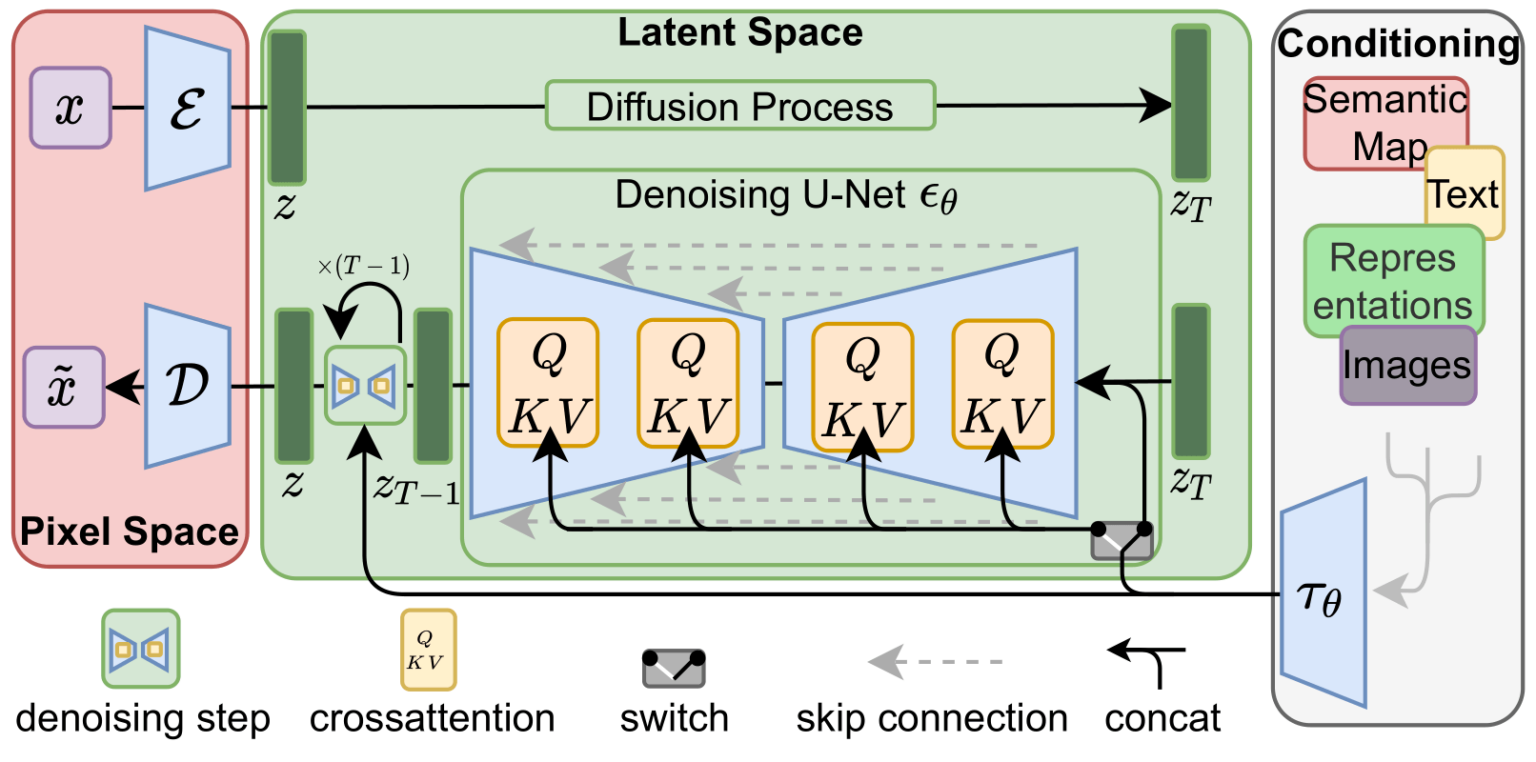
\includegraphics[width=\textwidth]{figures/2-sota/stable-diffusion.png}
    \caption[Stable diffusion architecture]{\textbf{Stable diffusion architecture} --- The Figure was taken from the original paper. On the top left, the original image $x$ is encoded with the \ac{AE}, and the diffusion process happens with the encodings. The text (or another data kind) is encoded with a transformer $\tau_{\theta}$, and these encodings are applied with attention to the denoising U-Nets. This denoising U-Net is applied $T$ times before the decoder transforms the encodings into an actual image in the pixel space again.}
    \label{fig:stable-diffusion}
\end{figure}
\subsubsection{GLIDE} \label{sec:glide}

The \acf{GLIDE} model is a state-of-the-art approach for generating high-fidelity synthetic images from free-form natural-language text prompts. The model is based on a guided diffusion-based approach, which is the first attempt by OpenAI at text-conditioned image generation using guided diffusion. The approach involves two types of guidance strategies during model training: classifier-free guidance~\cite{ho_classifier-free_2022}, which relies solely on the model's knowledge, and \ac{CLIP} guidance which uses a pre-trained \ac{CLIP} model~\cite{radford_learning_2021} to provide guidance based on caption matching.

The experimental results of the \ac{GLIDE} paper demonstrate several benefits of the proposed approach. Human evaluators preferred images generated with classifier-free guidance over \ac{CLIP} guidance regarding photorealism and caption similarity. Samples from the 3.5 billion parameter \ac{GLIDE} model were also found to outperform DALL-E (see Section~\ref{fig:dall-e}) samples according to human evaluations. Additionally, the model can perform text-driven image editing tasks beyond zero-shot image generation from text prompts. Text-driven image editing refers to editing existing images according to text prompts, such as changing attributes or objects within an image as directed by the text.

Despite its success, the \ac{GLIDE} model has some limitations. It fails to generate images for some complex or unusual text prompts. Moreover, the model's generation speed is slow, taking several seconds to generate one image on a flagship \ac{GPU}. Possible solutions to address these limitations include improving the model architecture, optimization techniques, and combining \ac{GLIDE} with faster \ac{GAN}-based methods.

\Acf{CLIP} refers to a model trained to determine if an image and text caption match. It consists of a transformer-based text encoder (see Section \ref{sec:transformers}) and a convolutional neural network-based image encoder (see Section \ref{sec:CNN}). The text encoder produces an embedding of the text, and the image encoder produces an embedding of the image. These embeddings are then compared, and during training, the model learns to produce similar embeddings for matching image-text pairs and dissimilar embeddings for mismatching pairs. This contrastive learning approach allowed CLIP to learn cross-modal understanding between text and images in an unsupervised manner. The pre-trained CLIP model can provide additional guidance to other text-to-image models, such as \ac{GLIDE}, by scoring how well-generated images match given text prompts.
\subsubsection{DALL-E 2} \label{sec:dall-e-2}

\textit{DALL-E 2} is a model proposed by researchers at OpenAI capable of generating images given a textual prompt~\cite{ramesh_hierarchical_2022}. This model can also modify given images, but this use case is not so interesting for the work present in this thesis.

The model consists of two blocks: the prior and the decoder. The prior converts captions into a lower-level representation, while the decoder turns this representation into an actual image.

They use \ac{CLIP} \cite{radford_learning_2021} and GLIDE (see Section~\ref{sec:glide}). For DALLE-2, the text is initially embedded using \ac{CLIP} embeddings. Then, the role of the prior is to translate these embeddings into embeddings related to an image and not the text itself. In other words, create an image representation with textual embeddings. For this, the researchers tried an \ac{AR} and a diffusion model. The diffusion one yielded better results (see Sections~\ref{sec:darn} and~\ref{sec:diffusion}). The decoder then takes the generated image representation and generates the image. The whole process can be seen in Figure \ref{fig:dall-e-2}.

\begin{figure}[ht]
    \centering
    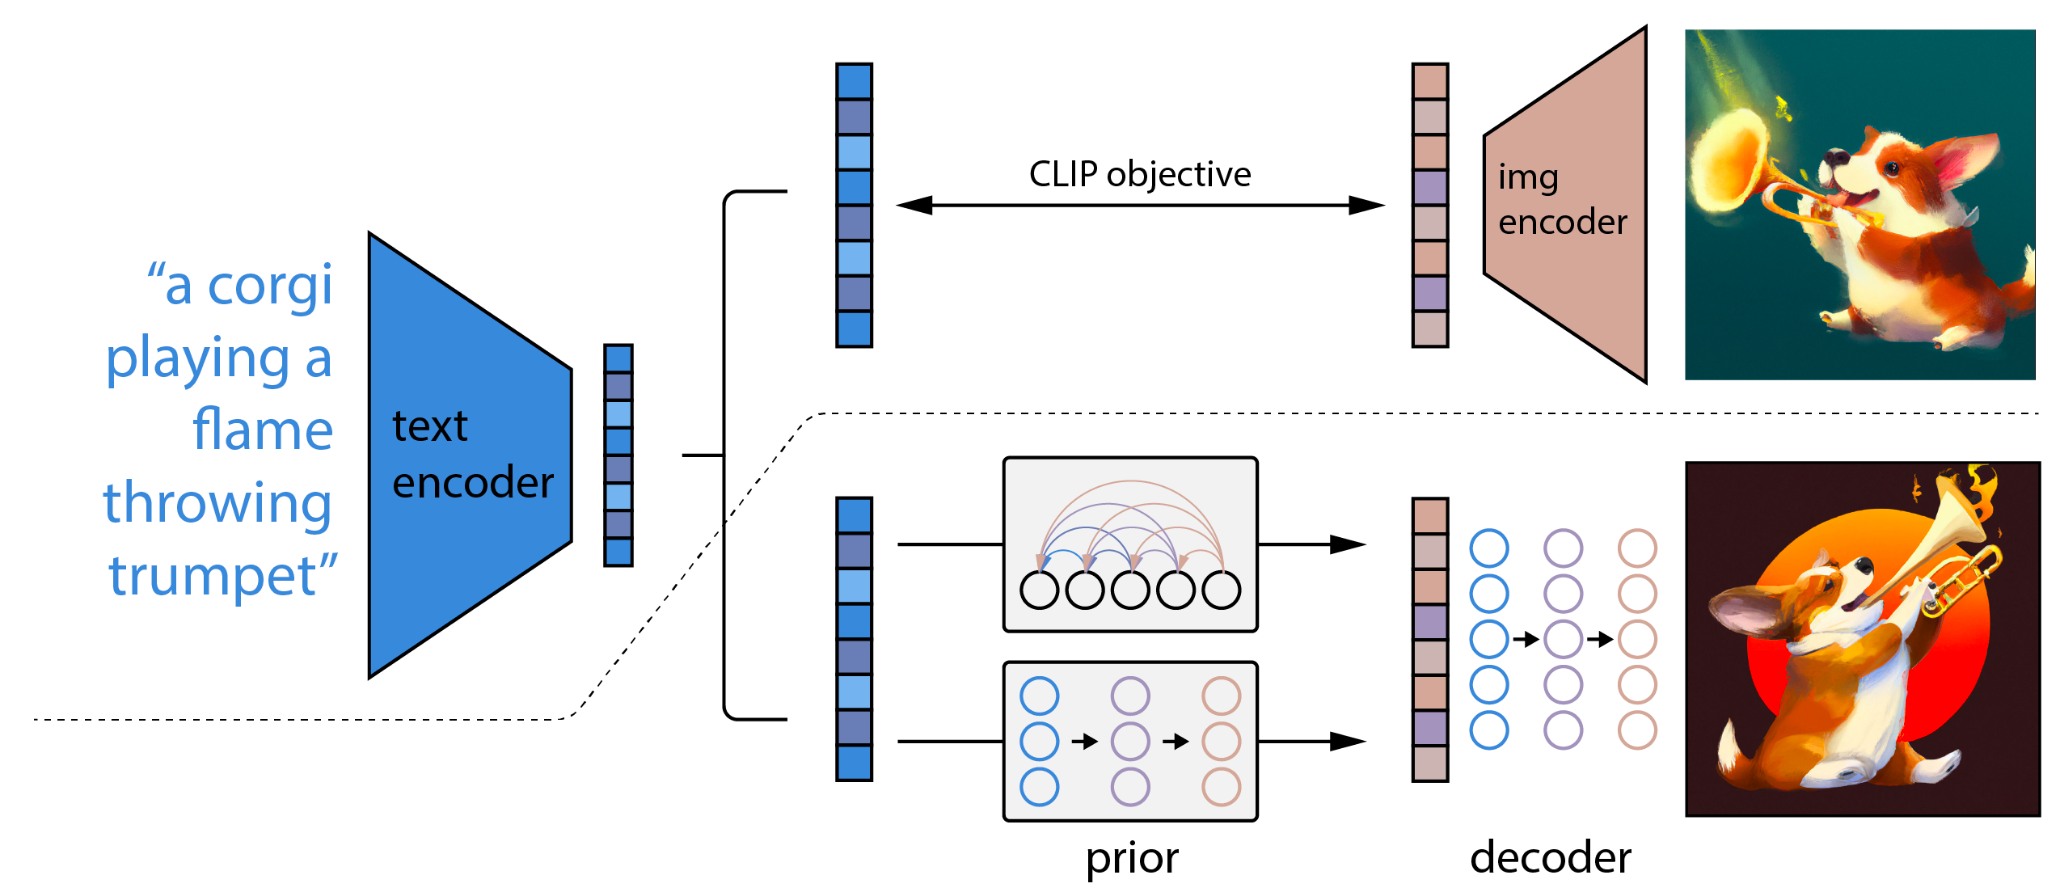
\includegraphics[width=\textwidth]{figures/2-sota/dall-e-2.png}
    \caption[DALL-E 2 architecture]{\textbf{DALL-E 2 architecture} --- The image was taken from the original paper. Above the dotted line, the \ac{CLIP} training process is depicted, where given textual and image embeddings, the \ac{CLIP} learns to translate one into the other. Below the dotted line, a text-to-image generation process is represented: a text embedding is first fed to the model that produces the image embedding. Then, this embedding is used to condition the diffusion model GLIDE which produces a final image.}
    \label{fig:dall-e-2}
\end{figure}

A model is also possible without the prior by passing the textual embeddings directly to the decoder. However, while the results were okay, they were way better with the generated image embeddings.

The decoder creates $64 \times 64$ images, but another network learns to upsample images until $1024 \times 1024$. Without this, generating high-resolution images with the decoder would make the whole operation incredibly heavy.

A significant problem of this model (and others presented here proposed by big companies) is that it needs hundreds of millions of images and an incredible amount of computation power to perform well. This highlights the importance of research toward openly accessible models such as stable diffusion (see Section~\ref{sec:stable-diffusion}).
\section{Related Work} \label{sec:related-work}

Traditionally, sound designers relied on manual labor to create audio, which involved recording and editing real-world sounds, mixing, and adding sound effects~\cite{sonnenschein_sound_2001}. Creating high-quality sounds is challenging, costly, and time-consuming, requiring specialized skills and resources. Hence, it engenders a notable impediment to the creation of soundscapes or any type of sound at scale~\cite{bernardes_seed_2016, strobl_sound_2006}, namely in light of its growing popularity and consumption within podcasts, movies, and video games.

Consumer data reported in 2021 showed compelling evidence regarding the listening habits of individuals within the United States of America. The findings indicate a substantial growth in podcast listenership over the past decade, with 41\% of Americans aged 12 or older having engaged with podcasts in the preceding month and 28\% within the last week. Moreover, at the beginning of the same year, a notable 68\% of Americans aged 12 and above had indulged in online audio consumption within the previous month, while 62\% had done so within the preceding week~\cite{research_infinite_2021}.

To overcome the aforementioned limitations, algorithmic audio generation has emerged as a promising solution that streamlines its creation altogether. Focusing on soundscapes, preceding 2018, prevailing models for their generation primarily revolved around statistical methods, featuring prominent employment of \ac{ML} techniques with feature engineering. For a comprehensive overview of techniques employed before the era of \ac{DL}, reference can be made to the review papers by Alias et al.\cite{alias_review_2016} and Kalonaris et al.\cite{kalonaris_computational_2018}. Noteworthy efforts at the feature engineering level are exemplified by Fernandez et al.~\cite{fernandez_ai_2013}, who represent sounds as high-level features, such as musical sheets, as an approach to generating musical sounds.

\Ac{DL} models for audio generation aim to produce high-quality audio signals by learning from existing audio data. Typically, these models consist of three main components: translation of the sound signal into a compressed representation, generation of a new representation from previous data, and translation back into an audio signal.

The first component of the model involves transforming the original sound signal into a Mel-spectrogram (or other) representation (see Section~\ref{sec:sound}), which is more compact and more accessible to process than the raw audio signal.

The second component involves generating new low-resolution representations from previous representations, such as spectrograms or feature vectors \cite{kong_hifi-gan_2020}. This is typically done using deep generative architectures. These models are trained on existing sound data to learn the target representation distribution and generate new, high-quality representations.

The final component of the model involves translating these representations back into an audio signal. These algorithms are called \textit{vocoders} (for more, see Section~\ref{sec:vocoders}). This component aims to produce high-quality audio signals that closely resemble the original sound data used to train the model.

The purpose of this section is to review the related work in this area. First, it examines the methods for generating traditional soundscapes, as described in Section~\ref{sec:trad-soundscape}. It then examines sound generation using machine learning. State-of-the-art models focus primarily on either using unsupervised sound generation techniques, as discussed in Section~\ref{sec:unsupervised-generation}, or generating sounds from internal representations, known as vocoders and discussed in Section~\ref{sec:vocoders}, or creating an end-to-end system, as discussed in Section~\ref{sec:end-to-end}.

\subsection{Traditional Soundscape Generation} \label{sec:trad-soundscape}

Feature engineering methods for soundscape generation typically adopt a threefold strategy to resynthesize (and extend) a short soundscape recording provided by the user:

\begin{enumerate}
    \item Segmentation,
    \item Feature extraction and modeling, and
    \item resynthesis of a given environmental sound.
\end{enumerate}

Statistical models adopting stochastic processes or pattern recognition methods were commonly applied to model and recreate a given soundscape recording with a degree of variation while maintaining its structure. Generated soundscapes relied on the similarity among audio segments to create smooth transitions~\cite{hoskinson_manipulation_2001}.

\subsubsection{Scaper}

Searching through the academic search engines, one finds that the most cited software for soundscape generation is \textit{Scaper} \cite{salamon_scaper_2017}.

Scaper is an open-source software library for soundscape generation designed to facilitate the creation of synthetic sound environments. It is a tool that allows users to simulate complex soundscapes, including urban, natural, and interior spaces, and investigate how various sound sources interact in these environments.

Scaper implements a modular soundscape generation framework based on basic sound-generating objects or ``sound sources''. These sound sources can represent simple sounds such as bird songs, human speech, or car horns, or more complex sounds like those produced by a crowd of people or a construction site. The user can specify the attributes of each sound source, such as its location, volume, and duration, and can adjust these parameters in real-time to create a dynamic soundscape.

One of the key features of Scaper is its ability to generate synthetic soundscapes that are diverse and statistically representative of real-world environments. To achieve this, the library implements various sound-generating algorithms that can be used to create sounds that are randomized yet realistic. For example, the library can generate sounds similar to real-world sources but with variations in volume, pitch, and timbre to avoid repetition and create a more diverse soundscape.

\subsubsection{SEED}

SEED is a system that addresses the formidable task of resynthesizing environmental sounds, such as city ambiances or nature scenes~\cite{bernardes_seed_2016}. SEED aims to provide a solution that not only extends the duration of environmental sounds but also provides precise control over the degree of variation in the output. This control over variation is critical in applications where maintaining the authenticity and coherence of the audio environment is essential.

SEED is built on a tri-partite architecture consisting of three main modules: segmentation, analysis, and generation. 

In the segmentation module, SEED performs the task of dividing the input audio into segments. This segmentation process is based on detecting spectral stability between frames. Spectral stability is a measure of how similar the frequency spectrum is between consecutive frames. When this stability falls below a certain threshold, it signals a change in the underlying sound source or event, prompting the placement of a segment boundary. This approach ensures that the resynthesized audio remains cohesive and retains its natural flow.

The Analysis module has two main processes. First, it extracts several audio features that capture both the sonic and temporal characteristics of the segments. These features are then clustered into a discrete ``dictionary'' of audio classes, effectively reducing the feature space to a finite set. At the same time, the module builds a transition table that records the sequences of these audio classes. This table is used to determine the probability that one class follows another.

In addition, the analysis module computes a concatenation cost matrix that quantifies how smoothly two segments can transition from one to the other. This matrix is computed by comparing the features at the segment boundaries. A lower cost indicates a smoother transition, while a higher cost indicates a more abrupt change.

In the Generation module, SEED generates new audio by searching for segment sequences that meet certain criteria. To achieve this, SEED references the transition table to determine viable next classes based on the current class in the audio sequence. It then assembles segments belonging to these classes and selects the one with the lowest concatenation cost. Notably, SEED applies a temporary cost penalty to recently selected segments to encourage diversity in the generated audio.

\subsubsection{Physics-Based Concatenative Sound Synthesis}

In the current development of virtual environments, the generation of audio content has been the subject of extensive research. One prominent approach in this area is \acf{CSS}, a method that creates novel auditory experiences by assembling segments of pre-existing sounds from a given database, often referred to as ``audio units''.

A recent scientific paper by Magalhães et al. presents an innovative \ac{CSS} framework based on physics-based principles for virtual reality~\cite{magalhaes_physics-based_2020}. This framework consists of two main components, namely the ``Capture Component'' and the ``Synthesis Component''.

The capture component of the framework is responsible for capturing essential data during interactions with virtual objects. This includes physics simulation data, haptic feedback data, position sensor data, and audio data. In particular, the physics data includes critical information such as collision points, velocities, impulses, and normals, among other parameters. The haptic and audio data are derived from real-world interactions with a variety of materials. This capture process culminates in the creation of a multimodal corpus of annotated audio units, which serves as the foundational resource for subsequent synthesis efforts.

The synthesis component of the framework uses the captured data to orchestrate the synthesis of auditory and haptic feedback by concatenating audio units extracted from the corpus. This unique mapping between physics data and audio units ensures congruence between user interactions and the resulting sensory feedback. For example, when a user applies a certain force and angle to interact with a virtual metal object, the synthesis component selects an audio unit recorded from a similar interaction with a real-world metal object.

At runtime, the framework relies on the target physics vectors to guide the selection of audio units, thus generating congruent auditory and haptic experiences. An overlap-add phase vocoder is used to concatenate the audio segments, while temporal repetition penalties are incorporated to ensure smooth transitions between these segments.
\subsection{Unsupervised Sound Generation} \label{sec:unsupervised-generation}

This Section focuses on models that address unsupervised or self-supervised training through learning sound features and their distributions without relying on explicit labels or annotations. In unsupervised sound generation, models learn from unlabeled audio data to capture underlying patterns and structures. This enables the generation of novel sound samples and the representation of latent features. This approach is particularly valuable when labeled datasets are scarce or expensive to acquire. Next, this discussion covers notable models in this area, selected based on their suitability for generating audio.

\subsubsection{WaveGAN} \label{sec:wavegan}

\Acp{GAN} have a notable impact on generating coherent images at the local and global levels, as discussed in Section~\ref{sec:gan}. A model based on \acp{GAN} called WaveGAN \cite{donahue_adversarial_2019} was proposed in 2019, to synthesize waveforms in an unsupervised manner. The model modifies the transposed convolution operation, used in \acp{DCGAN} for image generation, to capture waveform structure at different timescales.

WaveGAN modifies the transposed convolution operation in \acp{DCGAN}, expanding conventional \acp{GAN} to encompass image generation tasks and precisely capture the structure of audio signals of varying timescales. This model uses lengthier, one-dimensional filters of 25 units in place of two-dimensional filters with dimensions of $5 \times 5$. The model also upsamples each layer by a factor of 4, as is done in traditional \acp{DCGAN}. Despite these modifications, WaveGAN has the same number of parameters, numerical operations, and output dimensionality as \acp{DCGAN} have.

The experiments conducted on WaveGAN show that it can synthesize one-second slices of audio waveforms with global coherence, which is suitable for sound effect generation. The model also learns to produce intelligible words when trained on a small-vocabulary speech dataset without labels.

The success of WaveGAN in generating coherent audio signals demonstrates that \acp{GAN} can generate high-quality sounds. This work opens up new possibilities for unsupervised synthesis of raw-waveform audio, such as music and speech. It also suggests that \acp{GAN} can learn to capture the structure of signals across various timescales, which is crucial for generating realistic audio.

\subsubsection{Generative Transformer for Audio Synthesis}

In this work, Verma and Chafe~\cite{verma_generative_2021}, proposed in 2022, explore an alternative architecture using transformer networks (see Section~\ref{sec:transformers}), which have shown great success in sequential modeling tasks such as language translation.

The authors develop a generative transformer model for raw audio waveforms. The model is trained to autoregressively predict the next audio sample by attending over previous context samples. Specifically, the input waveform is split into overlapping frames and embedded into a latent space. A series of multi-headed causal self-attention layers then learn to focus on relevant parts of the input context to predict the subsequent sample distribution.

To retain information about the relative sample positions, positional encodings are added. Training deeper models is facilitated by layer normalization and residual connections. In a neural network, residual connections (also known as skip connections) enable the direct flow of information from one layer to subsequent layers. The use of residual connections helps to mitigate the vanishing gradient problem and allows for more effective gradient propagation during training. The inclusion of these connections enables the model to learn new representations at each layer and retain useful features from previous layers, resulting in improved performance and faster convergence. Self-attention provides the model with flexibility and frees it from the fixed topology of convolutions in other models such as WaveNet (Section~\ref{sec:wavenet}).

During training, previous samples are fed as input to the model to predict the next sample, optimized with cross-entropy loss (see Section~\ref{sec:cross-entropy}). The authors quantitatively evaluate next-step sample accuracy and find that the transformer architecture can outperform WaveNet baselines substantially.

\subsubsection{wav2vec 2.0}

The wav2vec 2.0 model comprises three essential components: a convolutional feature encoder, a Transformer network, and a quantization module. This model was originally introduced in the 2020 paper by Baevski et al. \cite{baevski_wav2vec_2020} and designed for speech generation tasks. For further details on the convolutional layer and the Transformer network, refer to Sections~\ref{sec:conv-layer} and \ref{sec:transformers}.

Quantization is the process of discretizing continuous values into a finite set of discrete symbols or codes, particularly in the context of generative models. This method is comparable to the technique used in the \ac{VQ-VAE} (refer to Section~\ref{sec:vq-vae}) In this technique, the input data is mapped to a limited number of discrete codebook entries.

For convolution, the feature encoder takes the raw audio waveform as input and generates a sequence of speech representations underlying it. This consists of several convolutional blocks, with each block including 1D temporal convolution and layer normalization. Wide kernels (\textit{e.g.,} 10ms) are used in the convolutions and progressively reduce the resolution of the input to extract hierarchical features.

The output of the feature encoder is fed into a transformer network to build contextualized representations. For encoding positional information specific to speech generation tasks, we use a convolutional layer instead of absolute positional embeddings. The self-attention mechanism enables each time step to consider all other time steps, thus capturing long-range dependencies in the sequence. Several Transformer layers extract higher levels of contextual abstraction.

A quantization module is applied to the output of the feature encoder. It discretizes the continuous latent representations into a finite inventory of speech units. Multiple codebooks are maintained, and concatenating selections from each codebook construct discrete units.

After pre-training on unlabeled speech, the model is fine-tuned on transcribed speech for speech recognition by adding a randomly initialized output layer. Various augmentations are used during fine-tuning to improve robustness.

The key innovations are the joint training of discrete speech units and contextualized representations in a completely self-supervised fashion. Experiments demonstrate strong performance even with just minutes of labeled data, highlighting the benefits of pre-training on large unlabeled corpora.

\subsubsection{SoundStream} \label{sec:soundstream}

SoundStream is a neural audio codec proposed in 2021 \cite{zeghidour_soundstream_2021} that can efficiently compress speech, music, and general audio. A codec is software or hardware that compresses and decompresses audio signals. The model architecture consists of a fully convolutional encoder/decoder network and a residual vector quantizer.

The fully convolutional encoder receives a time-domain waveform as input. It produces a sequence of embeddings at a lower sampling rate, which is then quantized by the \ac{RVQ}. The fully convolutional decoder then receives the quantized embeddings and reconstructs an approximation of the original waveform. Both the encoder and decoder use only causal convolutions, so the overall architectural latency of the model is determined solely by the temporal resampling ratio between the original time-domain waveform and the embeddings.

While there are similarities between SoundStream and a standard \ac{AE} (see Section \ref{sec:autoencoders}) in terms of the encoder-decoder architecture, SoundStream includes additional components such as the \ac{RVQ} and the use of structured dropout for variable bitrate compression.

A \acf{RVQ} is a vector quantization method. It is a variant of the traditional vector quantization method present, for instance, in \acp{VQ-VAE} (see Section \ref{sec:vq-vae}). In an \ac{RVQ}, the input data is first transformed into a lower-dimensional space using a neural network encoder. The resulting embeddings are then quantized using a codebook of fixed-size vectors, where each input embedding is assigned to the nearest codebook vector. However, instead of encoding the input embedding directly as the index of the assigned codebook vector, an \ac{RVQ} computes the difference between the input embedding and the assigned codebook vector, known as the residual. The residual is then quantized using a second codebook, and the indices of both codebook vectors are transmitted as the compressed representation.

Using residual vectors in \acp{RVQ} allows for better compression performance than traditional vector quantization methods. It captures the fine details of the input data that may be lost during quantization. In SoundStream, the \ac{RVQ} is used to quantify the embeddings produced by the fully convolutional encoder, enabling efficient audio compression at low bitrates while maintaining high audio quality.
\subsection{Vocoders} \label{sec:vocoders}

\Ac{DL} vocoders are neural network models that have the ability to generate artificial audio~\cite{mehrish_review_2023}. These models employ deep learning networks to learn the mapping between the input and waveform data directly. There is no reliance on any predefined model or feature extraction method. This approach has the ability to capture complex nonlinear relationships between input and output representations that are difficult to be modeled analytically.

There are different types of \ac{DL} vocoders, depending on the input and output representations they use. Some use Mel-spectrum features as conditioning inputs, while others do not require explicit features and directly generate raw waveform samples.

These models can achieve high quality and naturalness of audio synthesis, but they also face some challenges that limit their applicability. One challenge is the high computational cost of generating raw waveform samples at high sampling rates, which requires many computation and memory resources. This limits the scalability and efficiency of these models for real-time applications. Another challenge is the need for high-quality audio data with consistent annotations. This makes training these models with sufficient data diversity and coverage difficult. A third challenge is the generalization problem of these models, which tend to overfit the training data.

\subsubsection{WaveNet} \label{sec:wavenet}

\textit{WaveNet} is a generative neural network developed by DeepMind in 2016. It uses a unique architecture based on dilated causal convolutions to generate raw audio waveforms \cite{oord_wavenet_2016}. It implements the PixelCNN (see Section \ref{sec:pixelcnn}) model for sound and follows an \ac{AR} architecture (see Section \ref{sec:darn}) with the predictive distribution for each audio sample being conditioned on a window of previous ones.

WaveNet's structure allows it to process input sequences in parallel, enabling it to model long context dependencies, even with thousands of timesteps. It uses a series of dilated convolutional layers, where the dilation rate is increased with each layer, which effectively increases the receptive field of the network without increasing the number of parameters.

A dilated convolution happens when the filter is applied over an area larger than its length by skipping input values with a specific step \cite{oord_wavenet_2016}. This architecture can be seen in Figure \ref{fig:dilated-convolution}.

\begin{figure}[ht]
    \centering
    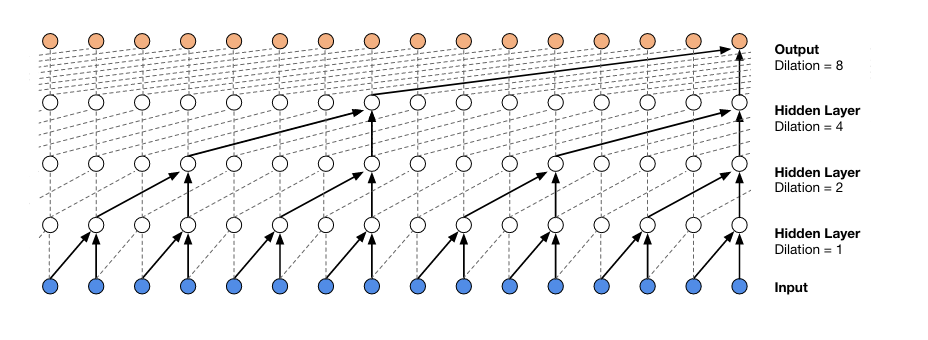
\includegraphics[width=\textwidth]{figures/2-sota/dilated-convolution.png}
    \caption[WaveNet]{\textbf{WaveNet} --- This illustration was taken from \cite{oord_wavenet_2016}. It shows the idea behind WaveNet, applying dilated convolutions to \ac{AR} models.}
    \label{fig:dilated-convolution}
\end{figure}

This structure enables WaveNet to capture long-range dependencies in the input sequence, which is crucial for generating high-quality audio. If an \ac{RNN} (see Section \ref{sec:rnn}) sees only one input sample at each time step, WaveNet has direct access to multiple input samples \cite{huzaifah_deep_2021}. For example, in speech generation, WaveNet can use its sizeable receptive field to model the relationship between a word spoken early in a sentence and its pronunciation later in the sentence.

WaveNet uses a softmax activation function at each output node to produce a probability distribution over the possible values at each time step. During training, the network is fed sequences of input data and their corresponding ground truth values. The model's parameters are adjusted so that its outputs match the ground truth as closely as possible.

WaveNet can use its trained parameters to generate new sequences by sampling from its output probability distribution during generation. This allows it to generate diverse and high-quality outputs, such as realistic human speech or written text, by combining its learned representations of the underlying data distribution with a small amount of randomness.

The input of WaveNet is usually a Mel-Spectrogram (or other representations), and the output is the sound signal.

WaveNet can be conditioned on, for instance, text for \ac{TTS} settings by feeding extra information about the text itself (\textit{e.g.} embeddings). If a model is not conditioned on text, it generates random sounds without any global structure behind it.

The results were astonishing. ``A single WaveNet can capture the characteristics of many different speakers with equal fidelity, and can switch between them by conditioning on the speaker identity. When trained to model music, we find that it generates novel and often highly realistic musical fragments.'' \cite{oord_wavenet_2016}.

Even though this model is good at learning the characteristics of sounds over brief periods, it struggles with global latent structure. They are also very slow for training and inferring \cite{tahiroglu_-terity_2020}.

%%%%%%%%%%%%%%%%%%%%%%%%%%%%%%%%%

\subsubsection{WaveNet Variants} \label{sec:wavenet-variants}

The WaveNet model has emerged as a powerful tool for generating high-quality audio waveforms, particularly for speech and music applications. However, its architecture, which employs dilated convolutions and deep residual networks, can be computationally intensive and challenging to train. To address these limitations, several WaveNet variants have been proposed in recent years that aim to reduce the complexity of the model while maintaining its effectiveness.

One such variant is \textbf{WaveRNN} \cite{kalchbrenner_efficient_2018}, which employs a single \ac{RNN} (see Section \ref{sec:rnn}) to approximate the dilated convolutions in WaveNet. This approach significantly speeds up training time while maintaining the quality of the generated audio. Another variant, FloWaveNet \cite{kim_flowavenet_2018}, employs a flow-based generative model (Section \ref{sec:flow-model}) that allows for efficient training with only one training stage while producing high-quality audio. Additionally, Fast WaveNet  \cite{paine_fast_2016} employs a caching mechanism to reduce the computational cost of the model while maintaining an \ac{AR} structure.

These WaveNet variants are unique in their architectures and training procedures but share the goal of making audio generation more efficient and accessible. While these models are primarily focused on speech and music generation, they can be adapted to other types of audio data. Ongoing research in this area may explore further optimization of these models, integration with other models, and application to new domains.

\subsubsection{MelGAN} \label{sec:melgan}

According to Kumar et al. in 2019, in their \textit{MelGAN} paper~\cite{kumar_melgan_2019}, audio generation with \acp{GAN} is possible although a challenging task (see Section \ref{sec:gan}). Previous studies in this field have encountered difficulties generating coherent raw audio waveforms using \acp{GAN}. Nonetheless, Kumar et al. demonstrate in their \textit{MelGAN} paper that introducing certain architectural changes makes it feasible to train \acp{GAN} to generate high-quality and coherent audio waveforms reliably.

The generator of MelGAN is a fully convolutional feed-forward network that takes a Mel-Spectrogram as input and generates a raw waveform as output. This approach allows for efficient and parallelized processing of audio data.

The decoder takes the waveform and decides whether it is a realistic sound. The decoder is not a single neural network but a multi-scale architecture with three discriminators (D1, D2, D3). These discriminators have identical network structures but operate on different audio scales. D1 operates on the scale of raw audio, while D2 and D3 operate on raw audio downsampled by a factor of 2 and 4, respectively. The use of multiple discriminators at different scales is motivated by the fact that audio has structure at different levels.

MelGAN proved itself way faster than other architectures such as WaveNet (see Section \ref{sec:wavenet}) with comparable results (for inference, roughly thirty-six thousand times faster than WaveNet), given its reduced number of parameters.


%%%%%%%%%%%%%%%%%%%%%%%%%%%%%%%%%

\subsubsection{GANSynth} \label{sec:gansynth}

\textit{GanSynth}, presented in 2019, \cite{engel_gansynth_2019} is a \ac{GAN} (see Section \ref{sec:gan}) that uses log-magnitude spectrograms and phases to generate coherent waveforms. Compared to directly generating waveforms with stridden convolutions, the use of spectrograms and phases has been shown to produce better results.

The study focuses on the NSynth \cite{engel_neural_2017} dataset, a collection of 300 000 musical notes from 1 000 different instruments.

The model first samples a random vector $z$ from a spherical Gaussian distribution. This vector is passed through a stack of transposed convolutions, which upsample and generate output data $x = G(z)$. This generated data is then fed into a discriminator network, which uses downsampling convolutions to estimate a divergence measure between the real and generated distributions.

The architecture of the discriminator network mirrors that of the generator, which allows for a more efficient training process. Optimizing the divergence measure allows the generator to produce spectrograms and phases that resemble actual musical notes more closely.

The study results demonstrate that \acp{GAN} outperform WaveNet (see Section \ref{sec:wavenet}) baselines on automated and human evaluation metrics and can efficiently generate several audio orders of magnitude faster than their \ac{AR} counterparts.

%%%%%%%%%%%%%%%%%%%%%%%%%%%%%%%%%

\subsubsection{HiFi-GAN}

Proposed in 2020, \textit{HiFi-GAN} \cite{kong_hifi-gan_2020} is a \ac{GAN} (see Section \ref{sec:gan}) model that combines efficiency and high-fidelity speech synthesis. HiFi-GAN achieves this by leveraging the periodic patterns inherent in speech audio, demonstrating that modeling these patterns is crucial for enhancing sample quality. The model includes a generator and two discriminators, trained adversarially, and two additional losses for improving training stability and model performance.

The generator is a fully \ac{CNN} (see Section~\ref{sec:CNN}) that takes Mel-Spectrograms as input and upsamples them through transposed convolutions, matching the temporal resolution of raw waveforms. The discriminators are the \ac{MSD} and a \ac{MPD}. \Ac{MSD} evaluates the audio sequence on different scales using a mixture of three convolutional sub-discriminators with different average pools. At the same time, \ac{MPD} consists of small sub-discriminators that capture different implicit structures of input audio by looking at different parts, accepting only equally spaced samples of input audio with different periods. 

HiFi-GAN's performance is evaluated using a subjective human evaluation (\ac{MOS}) on a single speaker dataset, which shows that the proposed method exhibits similarity to human quality. The model achieves a higher \ac{MOS} score than WaveNet (see Section \ref{sec:wavenet}).

Importantly, HiFi-GAN achieves this high-quality synthesis efficiently. Specifically, the model generates 22.05 kHz high-fidelity audio 167.9 times faster than real-time on a single V100 \ac{GPU}, demonstrating superior computational efficiency compared to AR and flow-based models. Moreover, a small-footprint version of HiFi-GAN generates samples 13.4 times faster than real-time on \ac{CPU} with comparable quality to an \ac{AR} counterpart.

\subsection{End-to-End Models} \label{sec:end-to-end}

Audio synthesis is the task of producing artificial audio from text or other kinds of data. Traditionally, audio synthesis systems consist of multiple stages, such as a data analysis frontend, a sound model, and an audio synthesis module. Building these components requires extensive domain expertise and may contain brittle design choices. Moreover, these components are usually trained separately on different objectives and datasets, which may introduce errors and inconsistencies in the final output. To overcome these limitations, end-to-end models have been proposed that directly learn the mapping between text (or other kinds of data) and audio waveform using deep neural networks. These models are presented in this Section.

Existing research establishes two main frameworks for end-to-end models: specialized models designed for a specific domain, and universal models aimed at broader applications. The table \ref{tab:end-to-end-audio-models} shows some examples of these models based on their type, input, output, model architecture, and type of conditioning. Specialized models target either speech or music synthesis, such as Char2wav and Jukebox. Researchers have developed different subsets of technologies within speech and music synthesis models, such as neural codec speech models and discrete diffusion models. Universal models, such as SampleRNN and AudioGen, can generate audio from various inputs and domains, such as text or raw audio seeds.

\begin{table}[ht]
\centering
\caption{A comparison of different end-to-end generative models for audio.}
\begin{tabularx}{\textwidth}{|l|l|X|X|X|}
\hline
\textbf{Model} & \textbf{Type} & \textbf{Input}            & \textbf{Output}                        & \textbf{Model Architecture}                                                      \\ \hline
Char2wav~\cite{sotelo_char2wav_2017}       & Speech        & Text prompt               & Raw audio waveform                     & Encoder-decoder with attention and neural vocoder                                \\ \hline
VALL-E~\cite{wang_neural_2023}         & Speech        & Text and acoustic prompt  & Raw audio waveform                     & Neural codec language model and neural vocoder                                   \\ \hline
Jukebox~\cite{dhariwal_jukebox_2020}        & Music         & Genre, artist, and lyrics & Raw audio waveform                     & Hierarchical VQ-VAE and autoregressive Transformer                               \\ \hline
Riffusion~\cite{forsgren_riffusion_2022}      & Music         & Text prompt               & Raw audio waveform                     & Neural codec language model based on discrete diffusion model and neural vocoder \\ \hline
MusicLM~\cite{agostinelli_musiclm_2023}        & Music         & Text prompt               & Raw audio waveform                     & Neural codec language model and neural vocoder                                   \\ \hline
SampleRNN~\cite{mehri_samplernn_2017}      & General       & None                      & Raw audio waveform                     & Hierarchical RNN and neural vocoder                                              \\ \hline
AudioLM~\cite{borsos_audiolm_2022}        & General       & Text prompt               & Raw audio waveform                     & Hybrid tokenization scheme with Transformer models and neural vocoder            \\ \hline
DiffSound~\cite{yang_diffsound_2022}      & General       & Text prompt               & Mel-spectrogram and raw audio waveform & VQ-VAE, discrete diffusion model, and neural vocoder                             \\ \hline
AudioGen~\cite{kreuk_audiogen_2023}       & General       & Text prompt               & Mel-spectrogram and raw audio waveform & Transformer-based generative model and neural vocoder                            \\ \hline
\end{tabularx}
\label{tab:end-to-end-audio-models}
\end{table}

%%%%%%%%%%%%%%%%%%%%%%%%%%%%%%%%%

\subsubsection{Text-to-Speech} \label{sec:tts}

\Acf{TTS} models are designed to convert written text into synthesized speech. These models use deep neural networks to directly learn the mapping between written text and audio waveform. Leveraging developments in \ac{NLP} and speech synthesis techniques, \ac{TTS} models have made significant progress in generating high-quality, human-like speech from text input. This Section examines some of the notable \ac{TTS} models that have been developed recently.

\paragraph{Char2Wav}

The Char2Wav model, proposed in 2017 \cite{rao_grapheme--phoneme_2015}, serves as a speech synthesis model comprising two distinct components: a reader and a neural vocoder. The reader takes text as inputs and produces a sequence of acoustic features as outputs. The neural vocoder then takes these acoustic features and generates raw waveform samples.

The reader is an attention-based recurrent sequence generator. It is a type of neural network that can generate a sequence of outputs based on a sequence of inputs. In this case, the inputs are text, and the outputs are acoustic features. The generator uses a bidirectional \ac{RNN} (see Section \ref{sec:rnn-variants}) as an encoder and a \ac{RNN} with attention as a decoder. The attention mechanism allows the model to focus on different parts of the input sequence as it generates the output.

Instead of using a traditional vocoder to generate the raw waveform samples, Char2Wav uses a learned parametric neural module. Specifically, it uses a conditional version of SampleRNN (see Section \ref{sec:samplernn} to learn the mapping from vocoder features to audio samples. This allows \textit{Char2Wav} to generate speech directly from the acoustic features without relying on a specific vocoder.

Although no formal proofs or analytical results are presented in this work, the proposed architecture is a significant breakthrough in speech synthesis. By demonstrating the effectiveness of using attention-based recurrent sequence generators and learned parametric neural modules, Char2Wav establishes a solid foundation for future research in this area.
\paragraph{VALL-E}

VALL-E is a language model developed by researchers at Microsoft for \ac{TTS} that treats \ac{TTS} as a conditional language modeling task~\cite{wang_neural_2023}. It generates text based on a given context, where the context in VALL-E is the acoustic tokens and phoneme prompts. VALL-E conditions on these inputs to produce the acoustic token sequence for speech synthesis.

VALL-E comprises two components: an audio codec that generates discrete acoustic tokens from speech waveforms and a neural language model that conditions these tokens and phoneme prompts to generate speech for unseen speakers in a zero-shot setting. The high-level architecture can be seen in Figure~\ref{fig:vall-e}.

\begin{figure}[ht]
    \centering
    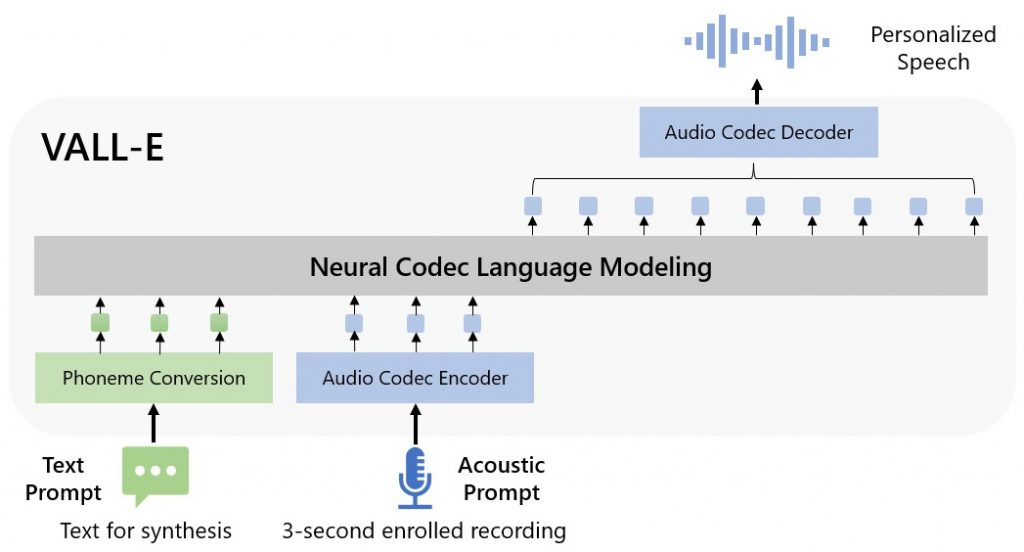
\includegraphics[width=\textwidth]{figures/2-sota/vall-e.jpg}
    \caption[VALL-E]{\textbf{VALL-E} --- The image was extracted from the source publication. It illustrates that both encodings derived from a linguistic prompt and an auditory prompt - provided via the codec encoder - are fed into a language model such as a transformer, and the resulting outputs are passed to the codec decoder to generate audio.}
    \label{fig:vall-e}
\end{figure}

The researchers trained VALL-E using the LibriLight dataset~\cite{kahn_libri-light_2020}, which consists of 60,000 hours of English speech from over 7,000 unique speakers. The proposed approach is robust to noise and generalizes well by leveraging a large and diverse dataset. Previous \ac{TTS} systems are typically trained with fewer data than VALL-E.

VALL-E's performance was evaluated on the LibriSpeech~\cite{panayotov_librispeech_2015} dataset, where all test speakers are unseen during training. VALL-E delivers high performance for speaker-adaptive \ac{TTS} in terms of speech naturalness and speaker similarity, as measured by comparative mean opinion score and similarity mean opinion score, respectively.

Qualitative analysis of VALL-E reveals several interesting findings. Firstly, VALL-E generates speech with diversity. As a result, the same input text can produce different speech outputs. This feature is important for downstream applications such as speech recognition, where diverse inputs with different speakers and acoustic environments are beneficial. The diversity of VALL-E makes it an ideal candidate for generating pseudo-data for speech recognition.

Another finding is that VALL-E maintains the acoustic environment of the prompt during speech synthesis. When the acoustic prompt has reverberation, VALL-E can synthesize speech with reverberation, whereas the baseline outputs clean speech. This can be attributed to VALL-E being trained on a large-scale dataset with diverse acoustic conditions, which allows it to learn acoustic consistency instead of only a clean environment during training.

Furthermore, VALL-E can preserve the emotion in the prompt during speech synthesis. The researchers selected acoustic prompts from the EmoV-DB dataset~\cite{adigwe_emotional_2018}, which contains speech with five emotions. VALL-E kept the exact emotion of the prompt in speech synthesis, even without fine-tuning on an emotional \ac{TTS} dataset.

VALL-E represents a significant advancement in \ac{TTS} technology, with its language model approach and use of audio codec codes as intermediate representations.

In summary, VALL-E is a language model-based \ac{TTS} system that utilizes audio codec codes as intermediate representations. It performs highly in speaker-adaptive \ac{TTS} and demonstrates exciting features such as speech diversity, acoustic environment consistency, and emotion preservation.

\subsubsection{Generative Music}

Generative music is created using generative techniques. End-to-end generative music models enable the production of new musical compositions without using predefined templates or samples, directly from textual or other data inputs. These models use \ac{DL} architectures to capture patterns and structures within different genres or styles of music, and can produce original pieces based on given prompts. This Section explores remarkable generative music models that demonstrate their ability to compose novel musical arrangements.

\paragraph{Jukebox}

Jukebox, a generative model for music that produces music with singing in the raw audio domain, was introduced by Dhariwal et al. in 2020 \cite{dhariwal_jukebox_2020}. The model tackles the long context of raw audio using a multiscale \ac{VQ-VAE} (see Section \ref{sec:ms-vq-vae}) to compress it to discrete codes and models those using \ac{AR} Transformers (see Section \ref{sec:transformers}).

The hierarchical \ac{VQ-VAE} architecture compresses audio into a discrete space, retaining the maximum amount of musical information at increasing compression levels. The model uses residual networks consisting of WaveNet-style (see Section \ref{sec:wavenet}) noncausal 1-D dilated convolutions, interleaved with downsampling and upsampling 1-D convolutions to match different hop lengths. Separate autoencoders with varying hop lengths are trained to maximize the amount of information stored at each level.

After training the \ac{VQ-VAE}, a prior $p(z)$ over the compressed space is learned to generate samples. The prior model is broken up as $p(z) = p(z_{top})p(z_{middle}|z_{top})p(z_{bottom}|z_{middle}, z_{top})$, and separate models are trained for the top-level prior $p(z_{top})$, and upsamplers $p(z_{middle}|z_{top})$ and $p(z_{bottom}|z_{middle}, z_{top})$. Autoregressive Transformers with sparse attention are used for modeling in the discrete token space produced by the \ac{VQ-VAE}.

Jukebox can generate high-fidelity and diverse songs with coherence for up to multiple minutes. It can be conditioned on the artist and genre to steer the musical and vocal style and on unaligned lyrics to make the singing more controllable. The model's release includes thousands of non-cherry-picked samples, model weights, and code.
\paragraph{Riffusion} \label{sec:riffusion}

Riffusion~\cite{forsgren_riffusion_2022} is an open-source model presented in 2022 that generates music clips from text prompts. The model is based on Stable Diffusion (see Section \ref{sec:stable-diffusion}). Riffusion fine-tunes Stable Diffusion to generate images of spectrograms, which can then be converted to music clips.

The authors use \ac{STFT} (see Section \ref{sec:stft}) to compute the spectrogram from audio. The \ac{STFT} is invertible so that the original audio can be reconstructed from a spectrogram. The authors use the Griffin-Lim algorithm~\cite{griffin_signal_1984} to approximate the phase when reconstructing the audio clip.

The authors use diffusion models (see Section \ref{sec:diffusion}) to condition the model's creations on a text prompt and other images, which is helpful for modifying sounds while preserving the structure of an original clip. The authors also use the denoising strength parameter to control how much to deviate from the original clip and towards a new prompt.

So, for inference, the model takes a text prompt as input. Then, the text is encoded into a latent representation using a text encoder. The model generates an image of a spectrogram from the latent representation using a modified version of Stable Diffusion; this is, the Stable Diffusion model fine-tuned for spectrograms. Finally, the generated spectrogram image is converted into an audio clip using the Griffin-Lim algorithm.
\paragraph{MusicLM} \label{sec:musiclm}

MusicLM is a generative model capable of synthesizing high-fidelity music characterized by realistic instrument timbres, accurate pitch, temporal patterns, and smooth transitions between notes based solely on textual descriptions of desired musical attributes (see Section~\ref{sec:musiclm}). The model extends the AudioLM framework for audio generation (see Section~\ref{sec:audiolm}) by incorporating text conditioning via the joint music-text model MuLan (see Section~\ref{sec:mulan}).

MusicLM employs a hierarchical modeling approach with two main stages: semantic modeling and acoustic modeling. The semantic modeling stage uses a Transformer decoder (see Section~\ref{sec:transformers}) to predict semantic tokens from the MuLan audio tokens. Using a separate Transformer decoder, the acoustic modeling stage then predicts acoustic tokens conditioned on both the MuLan audio tokens and predicted semantic tokens. This stage is subdivided into coarse and fine modeling substages to reduce the length of the token sequences, following the AudioLM approach.   

Overall, MusicLM leverages pre-trained audio encoders (SoundStream, w2v-BERT, and  MuLan) to obtain discrete acoustic and semantic tokens as input, after which hierarchical Transformer decoders first predict semantic tokens and then acoustic tokens when conditioned on MuLan text embeddings during synthesis. The hierarchical approach and use of semantic tokens aims to enable coherent long-term generation over extended durations.

MusicLM can generate coherent musical sequences up to 5 minutes in duration, constituting a notable achievement in the context of generative music models. The model captures various musical characteristics specified in textual prompts, including instrument timbre, melodic elements, and musical genre.

The model's performance was assessed using the MusicCaps dataset which comprises 5,500 pairs of music-texts that have been annotated by experts. The dataset includes diverse genres, instruments, and moods. The authors assert that this dataset thoroughly assesses the model's capability to generate various aspects of music from textual prompts. The evaluation metrics comprise human judgments of similarity between the generated outcomes and the prompts, as well as overall quality and others.    

The paper discusses potential limitations, including a proclivity for mode collapse and difficulty generating fine-grained structures over long sequences. However, further investigation is needed to probe the model's limitations and failure modes in greater depth.

In summary, MusicLM represents a promising generative model capable of synthesizing high-fidelity music from textual descriptions via shared embedding spaces and learned associations between text and music encodings, enabling it to capture diverse musical characteristics specified in textual prompts. The MusicCaps dataset provides a valuable means of evaluating the model's performance across various musical styles and prompts.

\subsubsection{General Text-to-Audio}

Text-to-audio systems have a wide range of applications beyond speech synthesis or generative music tasks. End-to-end models convert different forms of textual input into corresponding audio outputs. The outputs have diverse purposes, including sound effects generation, voice transformation, and environmental sound synthesis. These models provide flexible solutions for transforming text into realistic auditory experiences by training on large-scale datasets containing paired text-audio examples across various domains. This Section presents several text-to-audio approaches that demonstrate innovative methods of audio synthesis based on specific textual cues.

\paragraph{SampleRNN} \label{sec:samplernn}

\textit{SampleRNN} is a neural audio generation model proposed in 2017 that can produce high-quality audio samples from scratch \cite{mehri_samplernn_2017}. It uses a hierarchical structure of \acp{RNN} (see Section \ref{sec:rnn}) to model the probability distribution of audio waveforms at different temporal resolutions. The lowest \ac{RNN} operates on individual samples, while higher \acp{RNN} capture longer-term dependencies and structure. SampleRNN can learn from any audio data without any prior knowledge or labels.

The higher \acp{RNN} capture the longer-term dependencies by receiving inputs from lower \acp{RNN} at a lower sampling rate. This way, they can process longer audio sequences. The higher \acp{RNN} also use skip connections to directly access the outputs of lower \acp{RNN}, which helps to avoid vanishing gradients and preserve information across different levels of abstraction.

Each cell is a \ac{RNN} variant, such as \ac{GRU} (see Section \ref{sec:rnn-variants}) that takes as input a frame of audio samples from a lower \ac{RNN} and outputs a hidden state vector that encodes the long-term context of the audio. This output is passed upwards in the hierarchy to other \acp{RNN} that take it. Multiple layers are possible, each operating at a different temporal resolution. All the outputs are then inputted in the final level \ac{RNN}, whose output is the next audio sample based on the combined information from all hierarchy levels.
\paragraph{AudioLM} \label{sec:audiolm}

The framework called AudioLM was introduced by Borsos et al. in 2022 as a means for high-quality audio generation with long-term consistency~\cite{borsos_audiolm_2022}. In this representation space, the framework maps input audio to a sequence of discrete tokens and treats audio generation as a language modeling task. AudioLM achieves high-quality synthesis and long-term structure through a hybrid tokenization scheme. This scheme combines the discretized activations of a masked language model pre-trained on audio (semantic tokens) and the discrete codes produced by a neural audio codec (acoustic tokens).

The AudioLM framework consists of three main components:

\begin{enumerate}
	\item A \textit{tokenizer model} that maps the input audio $x$ into a sequence $y = \text{enc}(x)$ of discrete tokens from a finite vocabulary, with $T' < T$.
	\item A \textit{decoder-only Transformer language model} that operates on the discrete tokens $y$, trained to maximize the likelihood $\prod_{t=1}^{T'} p(y_t|y_{<t})$. The model predicts the token sequence $\hat{y}$ autoregressively at inference time.
	\item A \textit{detokenizer model} that maps the sequence of predicted tokens back to audio, producing the waveform $\hat{x} = \text{dec}(\hat{y})$.
\end{enumerate}

The tokenizer and detokenizer models are pre-trained and frozen before training the language model, simplifying the training setup. The number of tokens $T'$ is significantly smaller than $T$, allowing for increased temporal context size in the language model.

To reconcile the conflicting requirements of high-quality audio reconstruction and capturing long-term dependencies, AudioLM relies on a combination of acoustic and semantic tokens. Acoustic tokens are computed using SoundStream (see Section~\ref{sec:soundstream}). Semantic tokens are computed using w2v-BERT~\cite{chung_w2v-bert_2021}, a model for learning self-supervised audio representations. The semantic tokens enable long-term structural coherence while modeling the acoustic tokens conditioned on the semantic tokens enables high-quality audio synthesis.

AudioLM adopts a hierarchical approach by first modeling the semantic tokens for the entire sequence and then using these as conditioning to predict the acoustic tokens. AudioLM generates syntactically and semantically plausible speech continuations while maintaining speaker identity and prosody for unseen speakers when trained on speech without any transcript or annotation. The approach also extends beyond speech, generating coherent piano music continuations despite being trained without any symbolic representation of music.
\paragraph{DiffSound}

\textit{DiffSound} was presented in a paper, in 2022, that displays a novel text-to-sound generation framework that uses a text encoder, a \ac{VQ-VAE}, a decoder, and a vocoder. The framework takes text as input and outputs synthesized audio corresponding to the input text. The decoder, in particular, is a critical component of the framework, and the paper focuses on designing a suitable decoder, calling it \textit{DiffSound} \cite{yang_diffsound_2022}.

DiffSound is a diffusion decoder (Section \ref{sec:diffusion}) based on the discrete diffusion model. DiffSound predicts all Mel-Spectrogram tokens in one step and then refines the predicted tokens in the next step, resulting in better-predicted results after several steps. It not only produces better text-to-sound generation results compared to an \ac{AR} decoder, but it is also faster, with a generation speed five times faster than an \ac{AR} decoder.

The entire framework acts as this: First, the text is encoded into embeddings using a model like a transformer (Section \ref{sec:transformers}). Then, this representation conditions the generation of spectrogram embeddings using diffusion (the DiffSound model). These embeddings are then passed through the pretrain \ac{VQ-VAE} decoder to generate the spectrogram. The spectrogram runs through a vocoder (Section \ref{sec:vocoders}) to generate the waveform. In the original text, the vocoder used was the MelGAN (see Section \ref{sec:melgan}). This process can be seen in Figure \ref{fig:diffsound}.

\begin{figure}[ht]
    \centering
    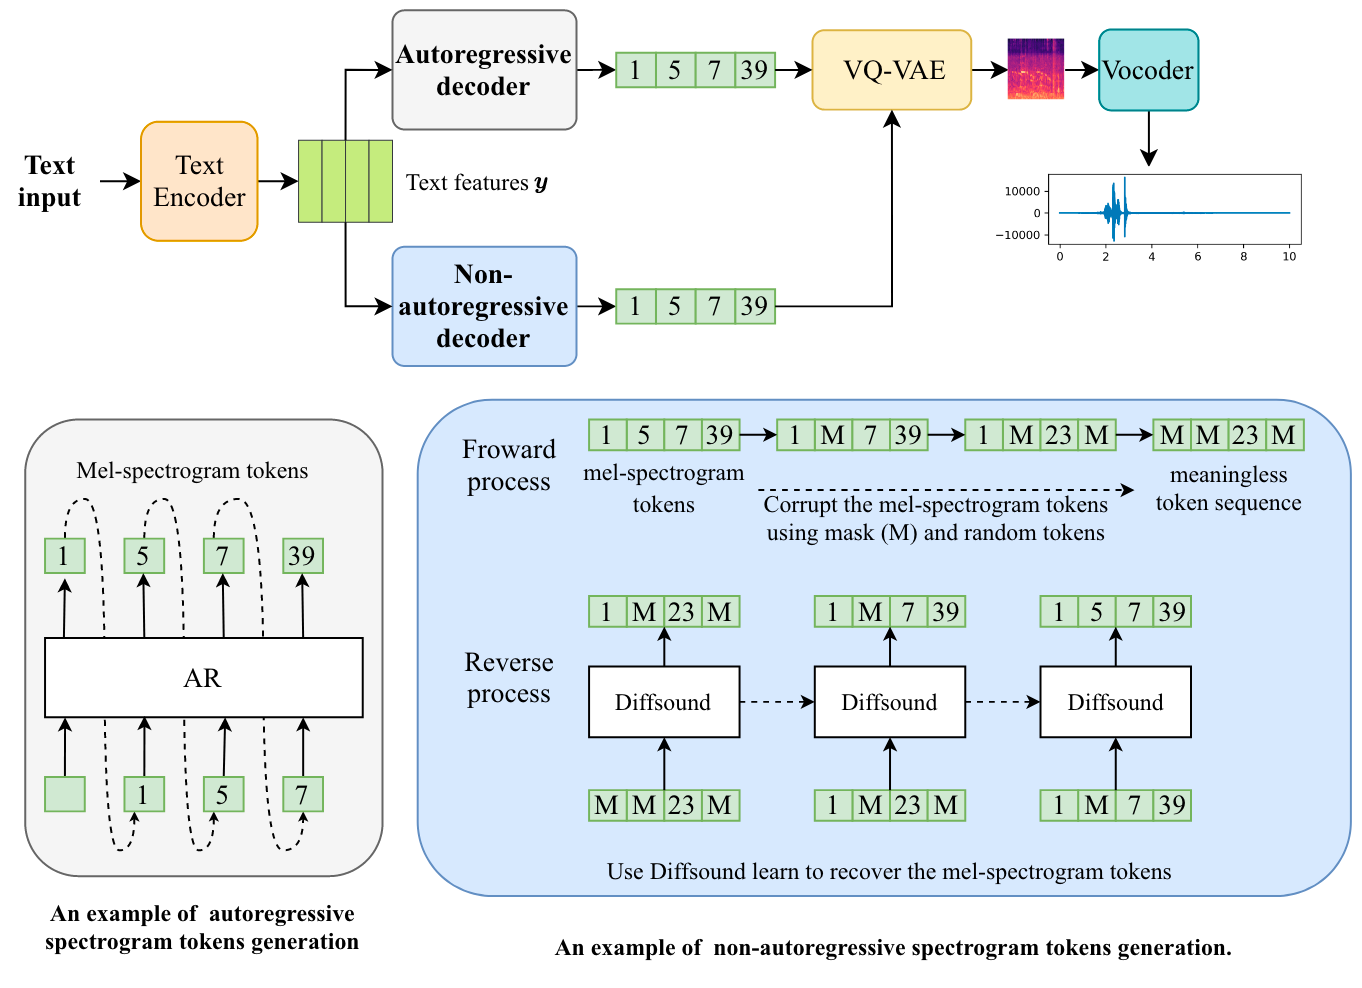
\includegraphics[width=\textwidth]{figures/2-sota/diffsound.png}
    \caption[DiffSound framework]{\textbf{DiffSound framework} --- This illustration was taken from the original paper. At the top, the general framework is present. Two decoders are present, but only one of them is used. The decoder results in a set of latent features. These features are passed to the decoder of the \ac{VQ-VAE} that generates a Mel-Spectrogram (the square with red and blue tones) that, through a vocoder, generates a sound. The two bottom images represent the two decoders. One is a \ac{DARN} (see Section \ref{sec:darn}), the other works with diffusion.}
    \label{fig:diffsound}
\end{figure}
\paragraph{AudioGen} \label{sec:audiogen}

In 2023, Kreuk et al.~\cite{kreuk_audiogen_2023} proposed AudioGen, an auto-regressive generative model that generates audio samples conditioned on text inputs. The model comprises two primary stages: (i) learning a discrete representation of the raw audio using an \ac{AE} method and (ii) training a Transformer language model (see Section~\ref{sec:transformers}) over the learned codes obtained from the audio encoder, conditioned on textual features. During inference, the model samples from the language model generate a new set of audio tokens given text features, which can then be decoded into the waveform domain using the decoder component.

To address the challenge of text-to-audio generation, the authors propose an augmentation technique that mixes different audio samples to train the model to separate multiple sources internally. Furthermore, the authors explore the use of multi-stream modeling for faster inference, allowing the use of shorter sequences while maintaining a similar bitrate and perceptual quality. The proposed method outperforms evaluated baselines over both objective and subjective metrics. Additionally, the authors extend the proposed method to conditional and unconditional audio continuation, demonstrating its ability to generate complex audio compositions.


